% ==============================================================================
\chapter{The Timepix3 beam telescope}
\label{ch:Telescope}
% ==============================================================================  

%% --------------------------------------------- %% 

Testing in a high energy beam is a crucial step in the R\&D for the
pixel detector sensors and readout chips. Test beam data are used at
various stages of the development for evaluating the performance of a
prototype in addition to simulations tools like TCAD and
\textsc{Geant4}.

A telescope is used to reconstruct the tracks of the particles going
through its planes. The track position is then extrapolated on the
Device Under Test (DUT). This allows to compare the position of the
hit on the DUT with the reconstructed track and extract the position
and time resolutions as well as the efficiency of the device.

For the CLIC vertex detector R\&D, the CLICdp Timepix3 telescope is
used as a beam reference. This chapter gives an overview of the
components of the Timepix3 telescope and its tracking performance. The
telescope is implemented in AllPix simulations
(c.f. \cref{sec:AllPix}) and its performance is compared to the data
taken at the CERN SPS~\cite{SPS}. Finally, the tracking resolution on
the DUT is extracted in simulations using the Monte Carlo information.

%% --------------------------------------------- %%
\section{Experimental setup at the CERN SPS}
\label{sec:CERN_SPS}

The telescope is placed at the H6 beam~\cite{H6Beamline} of the CERN
SPS typically operated with a $120\,\gev$ pion beam. The assemblies
listed in \cref{tab:Timepix3Assemblies} are tested as DUTs using this
telescope. The beam is configured in such a way to have around
$1-5 \times 10^6$ particles per five-second spill. The telescope
planes are positioned in a way to give the best tracking resolution
for the given beam energy taking into account multiple scatterings and
mechanical constraints. The optimisation is performed based on a
global $\chi^2$-minimisation
~\cite{Zarnecki:2007yu,OnlineTelescopePositioning}. The resulting
optimal configuration implies a narrow spacing of all detector planes.


%% --------------------------------------------- %%
\section{Components of the telescope}

%% --------------------------------------------- %%
\subsection{Coordinates system}
A Cartesian right-handed coordinate system is chosen to describe the
geometry of the telescope. The z-direction is along the beam as shown
in \cref{fig:TPX3Telescope} and the y-direction points vertically in
the up direction.

%% --------------------------------------------- %%
\subsection{Sensors and mechanics}
\label{sec:Telescope_sensors_mechanics}

The telescope consists of six planes of Timepix3
ASICs~\cite{Timepix3Poikela} bump bonded to $300\,\micron$ thick
p-in-n planar sensors (produced by Canberra) as shown in
\cref{fig:TPX3Telescope}. The sensors are depleted at a bias voltage
of 30~V and nominally operated at 50~V. The Timepix3 readout chip
threshold is set to $\sim1000$ electrons. The planes are tilted by
$9\degrees$ around the x and y axes~\cite{Akiba:2013yxa}. Given the
pixel pitch and the sensor thickness, this angle mainly leads to
clusters of three pixels. Combining the TOT information, the
reconstructed hit position provides sub-pixel resolution on the
telescope planes. This leads to a tracking resolution of
$\sim$$2\,\micron$ on the DUT.


\begin{figure}[htbp]
  \centering
  \begin{tikzpicture}
    \node[anchor=south west,inner sep=0] (image) at
    (0,0){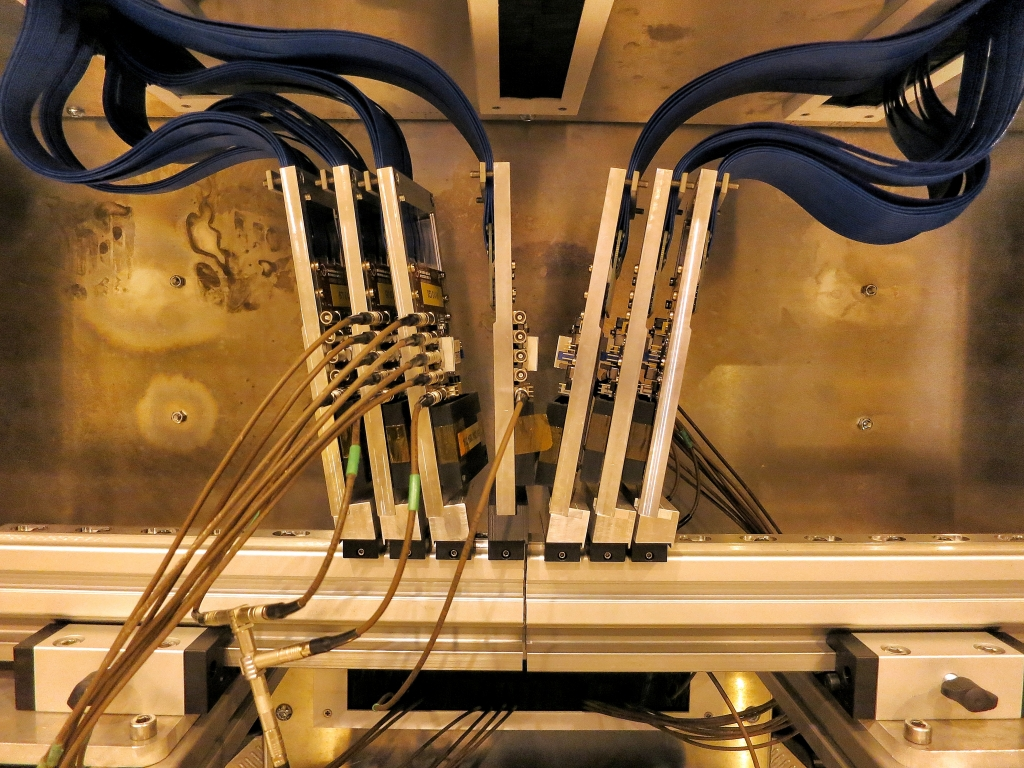
\includegraphics[width=0.6\textwidth]{ActiveEdge/Timepix3Telescope.jpeg}};
    \begin{scope}[x={(image.south east)},y={(image.north west)}]
      \node[above, color=white] at (0.5, 0.85) {Device Under Test};
      \node[above, color=white] at (0.5, 0.78) {(\textbf{DUT})};

      \draw[->, very thick, color=black](0.75, 0.42) -- (0.25, 0.42);
      \node[right, color=black] at (0.77, 0.42) {\textbf{Beam}};

      \draw[<->, very thick, color=black](0.33, 0.25) -- (0.66, 0.25);
      \node[below, color=black] at (0.5, 0.25) {\textbf{152~mm}};

      \node[color=black] at (0.64, 0.32) {\textbf{0}};
      \node[color=black] at (0.6, 0.32) {\textbf{1}};
      \node[color=black] at (0.55, 0.32) {\textbf{2}};

      \node[color=black] at (0.44, 0.32) {\textbf{3}};
      \node[color=black] at (0.39, 0.32) {\textbf{4}};
      \node[color=black] at (0.35, 0.32) {\textbf{5}};
      
      % \draw[help lines,xstep=.1,ystep=.1] (0, 0) grid (1,1);
      % \foreach \x in {0,1,...,9} { \node [anchor=north] at (\x/10,0) {0.\x}; }
      % \foreach \y in {0,1,...,9} { \node [anchor=east] at (0,\y/10) {0.\y}; }
      
    \end{scope}
  \end{tikzpicture} 
  \caption{The Timepix3 beam reference telescope with six tilted
    planes for the tracking and the DUT in the middle inserted
    perpendicular to the beam direction. The telescope planes
    numbering convention is also shown.}
  \label{fig:TPX3Telescope}
\end{figure}

The position of the telescope planes and the DUT along the beam axis
using the convention as described in \cref{fig:TPX3Telescope} is given
in \cref{tab:planePos}. The positions correspond the position of the
center of the sensors.

\begin{table}[htbp]
  \centering
  \caption{The position of the telescope planes and the DUT along the
    beam axis.}
  \label{tab:planePos}
  \begin{tabular}{ c c }
    \toprule
    Plane number & Position [mm] \\
    \midrule
    0 & 0 \\
    1 & 23.5 \\
    2 & 47 \\
    DUT & 77 \\
    3 & 106.5 \\
    4 & 128 \\
    5 & 151.5 \\
    \bottomrule
  \end{tabular}
\end{table}

The mechanical support for the telescope planes are optimised in order
to reduce multiple scattering and therefore improve the tracking
resolution. The Timepix3 assemblies are mounted on a PCB as shown in
\cref{fig:Timepix3board_PCB}. An aluminum support frame is used to
hold the PCB. To protect the sensors from light exposure, an ABS
plastic cover is used with a thickness of 2~mm and placed at a
distance of 10~mm away from the PCB (in black in
\cref{fig:TPX3Telescope}). \cref{tab:TPX3TelescopeMaterial} describes
the material (with their thicknesses and radiation lengths) seen by
the particles for each telescope plane. The PCB stacks up eight layers
of copper interlacing with Isola IS410 type material with an average
fill factor of $75\%$ for copper. Behind the PCB, a layer of Copper is
used for the cooling of the chip. The total material of a telescope
plane is estimated to correspond to $\sim4\%$~X\textsubscript{0}.

\begin{table}[htbp]
  \centering
  \caption{The material in each telescope plane contributing to the
    multiple scatterings of the traversing particles. X refers to the thickness and X\textsubscript{0} to the radiation
    length.}
  \label{tab:TPX3TelescopeMaterial}
  \begin{tabular}{l c c c}
    \toprule
    Material & X [mm] & X\textsubscript{0} [mm] & X/X\textsubscript{0} [$\%$] \\
    \midrule
    Cooling material for the chip (Cu) & 0.1 & 14.4 & 0.69 \\
    Isola IS410 in the PCB & 1.475 & 167.6 & 0.88 \\
    Copper in the PCB & 0.125 & 14.4 & 0.87 \\
    ASIC (Si) & 0.7 & 93.7 & 0.75\\
    Sensor (Si) & 0.3 & 93.7 & 0.32\\ 
    Sensor cover (ABS plastic) & 2 & 406.4 & 0.49 \\ \hline
    Total & & & 4 \\
    \bottomrule
  \end{tabular}
\end{table}

%% --------------------------------------------- %%
\subsection{Data acquisition system}
The SPIDR readout system, as described in \cref{sec:TimepixReadout},
is used for the data acquisition of the Timepix3 telescope planes. The
Timepix3 readout ASICs are operated with the data-driven
zero-suppressed readout mode. This system allows to record the data
from all the particles from the SPS spill without dead time. The data
is processed offline using the EUTelescope framework as described in
\cref{sec:recoSoft}.


%% --------------------------------------------- %%
\section{The telescope performance}
\label{sec:telescopePerformance}

The telescope is simulated with the \textsc{Geant4}-based AllPix
simulation framework (c.f. \cref{sec:AllPix}). This allows for a
better understanding of the telescope performance, extraction of the
tracking resolution on the DUT and comparison to data. Since AllPix
gives access to the Monte Carlo position (MC position) of the hits,
the true tracking resolution can be obtained by comparing the MC
position with the reconstructed track or hit positions.

\subsection{Timepix3 telescope simulation in AllPix}
In the simulations, the geometry of the telescope is defined in a
realistic way by taking into account the positions and the rotations
of the telescope planes, the thickness of the sensors and the pixel
pitch. \cref{fig:Timepix3Telescope_Allpix} shows the geometry of the
telescope as implemented in AllPix.

The mechanical supports for the telescope planes are implemented using
the material as described in \cref{tab:TPX3TelescopeMaterial}.

% \textsc{Geant4} provides the class \textsc{G4Material} which describes
% the macroscopic properties of the material used in simulations and
% contains all the relevant information on its constituent elements. The
% density and the radiation length of the material are the two main
% properties to be considered for the simulations. \textsc{Geant4}
% already provides a material database for all the standard material
% such as copper and silicon. For the Isola IS410, the material
% G4\_BONE\_COMPACT\_ICRU has the closest radiation length and
% density. For the sensor covers in ABS plastic, their constituent
% elements
% (C\textsubscript{8}H\textsubscript{8}~C\textsubscript{4}H\textsubscript{6}~C\textsubscript{3}H\textsubscript{3}N)
% have been implemented as a \textsc{G4Material} in the simulations to
% obtain the correct density and radiation length.

\begin{figure}[htbp]
  \centering
  \begin{tikzpicture}
    \node[anchor=south west,inner sep=0] (image) at
    (0,0){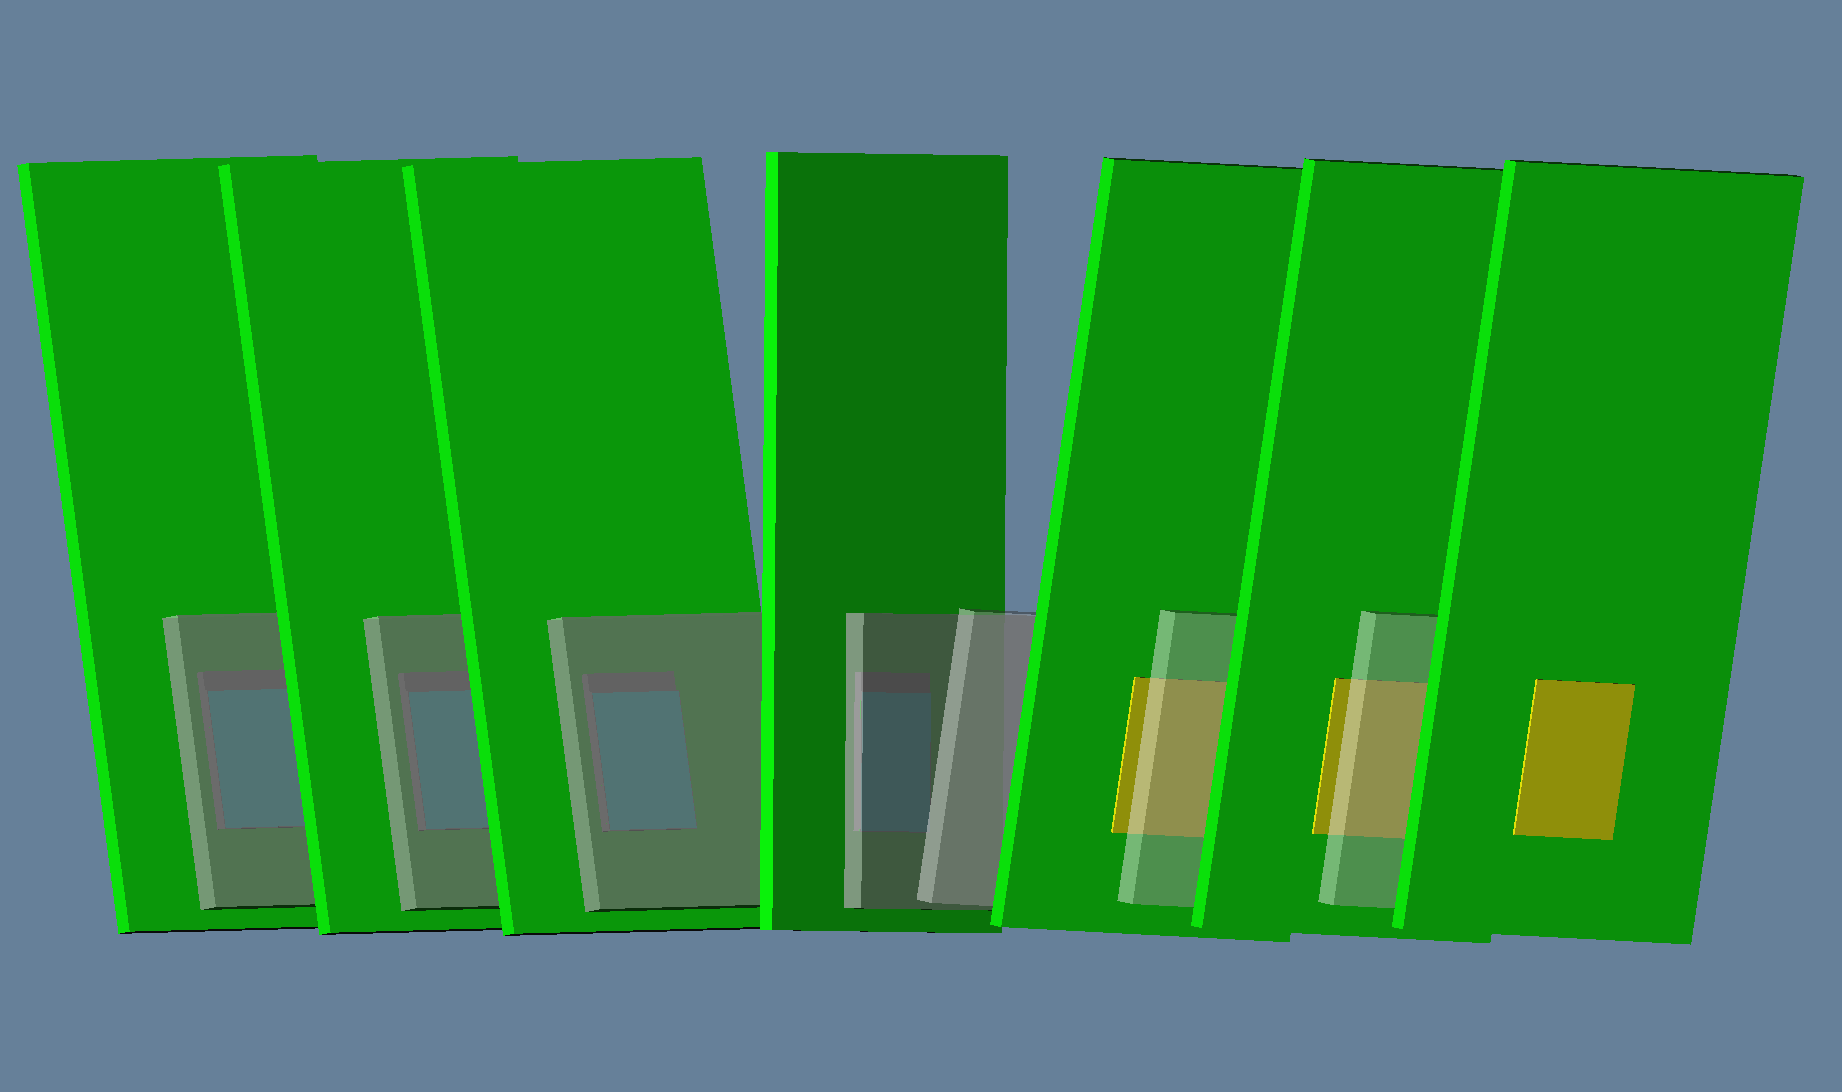
\includegraphics[width=0.6\textwidth]{figures/Telescope/AllpixTelescope.png}};
    \begin{scope}[x={(image.south east)},y={(image.north west)}]
      
      \draw[->, very thick, color=black](0.8, 0.9) -- (0.25, 0.9);
      \node[above, color=black] at (0.5, 0.91) {\textbf{Beam}};
      
      \node[above, color=black] at (0.9, 0.05) {\footnotesize{Plane 0}};
      \node[above, color=black] at (0.75, 0.05) {\footnotesize{Plane 1}};
      \node[above, color=black] at (0.6, 0.05) {\footnotesize{Plane 2}};
      \node[above, color=black] at (0.48, 0.05) {DUT};
      \node[above, color=black] at (0.35, 0.05) {\footnotesize{Plane 3}};
      \node[above, color=black] at (0.2, 0.05) {\footnotesize{Plane 4}};
      \node[above, color=black] at (0.07, 0.05) {\footnotesize{Plane 5}};

      \node[above, color=black] at (0.35, 0.7) {Sensor cover};
      \draw[->, color=black](0.35, 0.7) -- (0.35, 0.45);
      \node[above, color=black] at (0.9, 0.7) {Cooling};
      \draw[->, color=black](0.85, 0.7) -- (0.85, 0.4);

      %% \draw[help lines,xstep=.1,ystep=.1] (0, 0) grid (1,1);
      %% \foreach \x in {0,1,...,9} { \node [anchor=north] at (\x/10,0) {0.\x}; }
      %% \foreach \y in {0,1,...,9} { \node [anchor=east] at (0,\y/10) {0.\y}; }
      
    \end{scope}
  \end{tikzpicture} 
  \caption{The Timepix3 beam reference telescope implemented in AllPix
    with six tilted planes for the tracking and the DUT in the middle
    inserted perpendicular to the beam direction. The telescope planes
    numbering convention is also shown in this figure.}
  \label{fig:Timepix3Telescope_Allpix}
\end{figure}


A digitiser for the Timepix3 readout chips bump-bonded to planar
sensors is defined in AllPix. It simulates the silicon physics by
calculating the drift and diffusion at each \textsc{Geant4} step as
described in \cref{sec:allpix_digitisation}. The contribution of the
generated charge by drift and diffusion in the hit pixel and its
neighbouring pixels is calculated for each step. All contributions
add-up and the charge in each pixel is calculated. The electronic
noise of the Timepix3 ASIC defined by a Gaussian distribution of width
$\sim80$ electrons sums up to the charge in each pixel. The readout
threshold as obtained from the threshold calibration for the
corresponding device is applied to each pixel and finally, the
pixel-by-pixel TOT calibration (see \cref{sec:EnergyCalibration}) is
applied to convert the energy deposition in TOT. The operation
parameters as described in \cref{sec:Telescope_sensors_mechanics} are
used for the AllPix simulations of the sensors of the telescope
planes.

The \textsc{Geant4} General Particle Source (GPS) is used for the
simulation of $120\,\gev$ pions. The GPS generates a parallel beam
with a transverse (radial) standard deviation of 5~mm.

The spread of the simulated track angles due to multiple scattering is
shown in \cref{fig:MCbeamAngleDistr}. A scattering of 0.1~mrad causes
a displacement of up to $\sim3\,\micron$ over a distance of 30~mm. The
angles $\phi$ (in horizontal direction) and $\theta$ (in vertical
direction) are given as:

\begin{equation}
  \phi=arctan{{x_2-x_{DUT}} \over {z_2-z_{DUT}}} \; ,
  \label{eq:beamAnglePhi}
\end{equation}

\begin{equation}
  \theta=arctan{{y_2-y_{DUT}} \over {z_2-z_{DUT}}} \; ,
  \label{eq:beamAngleTheta}
\end{equation}

where $x, y$ and $z$ are the MC positions of the hits on the planes 2
and the DUT.

\begin{figure}[htbp] \centering
  \begin{subfigure}[b]{0.45\textwidth}
    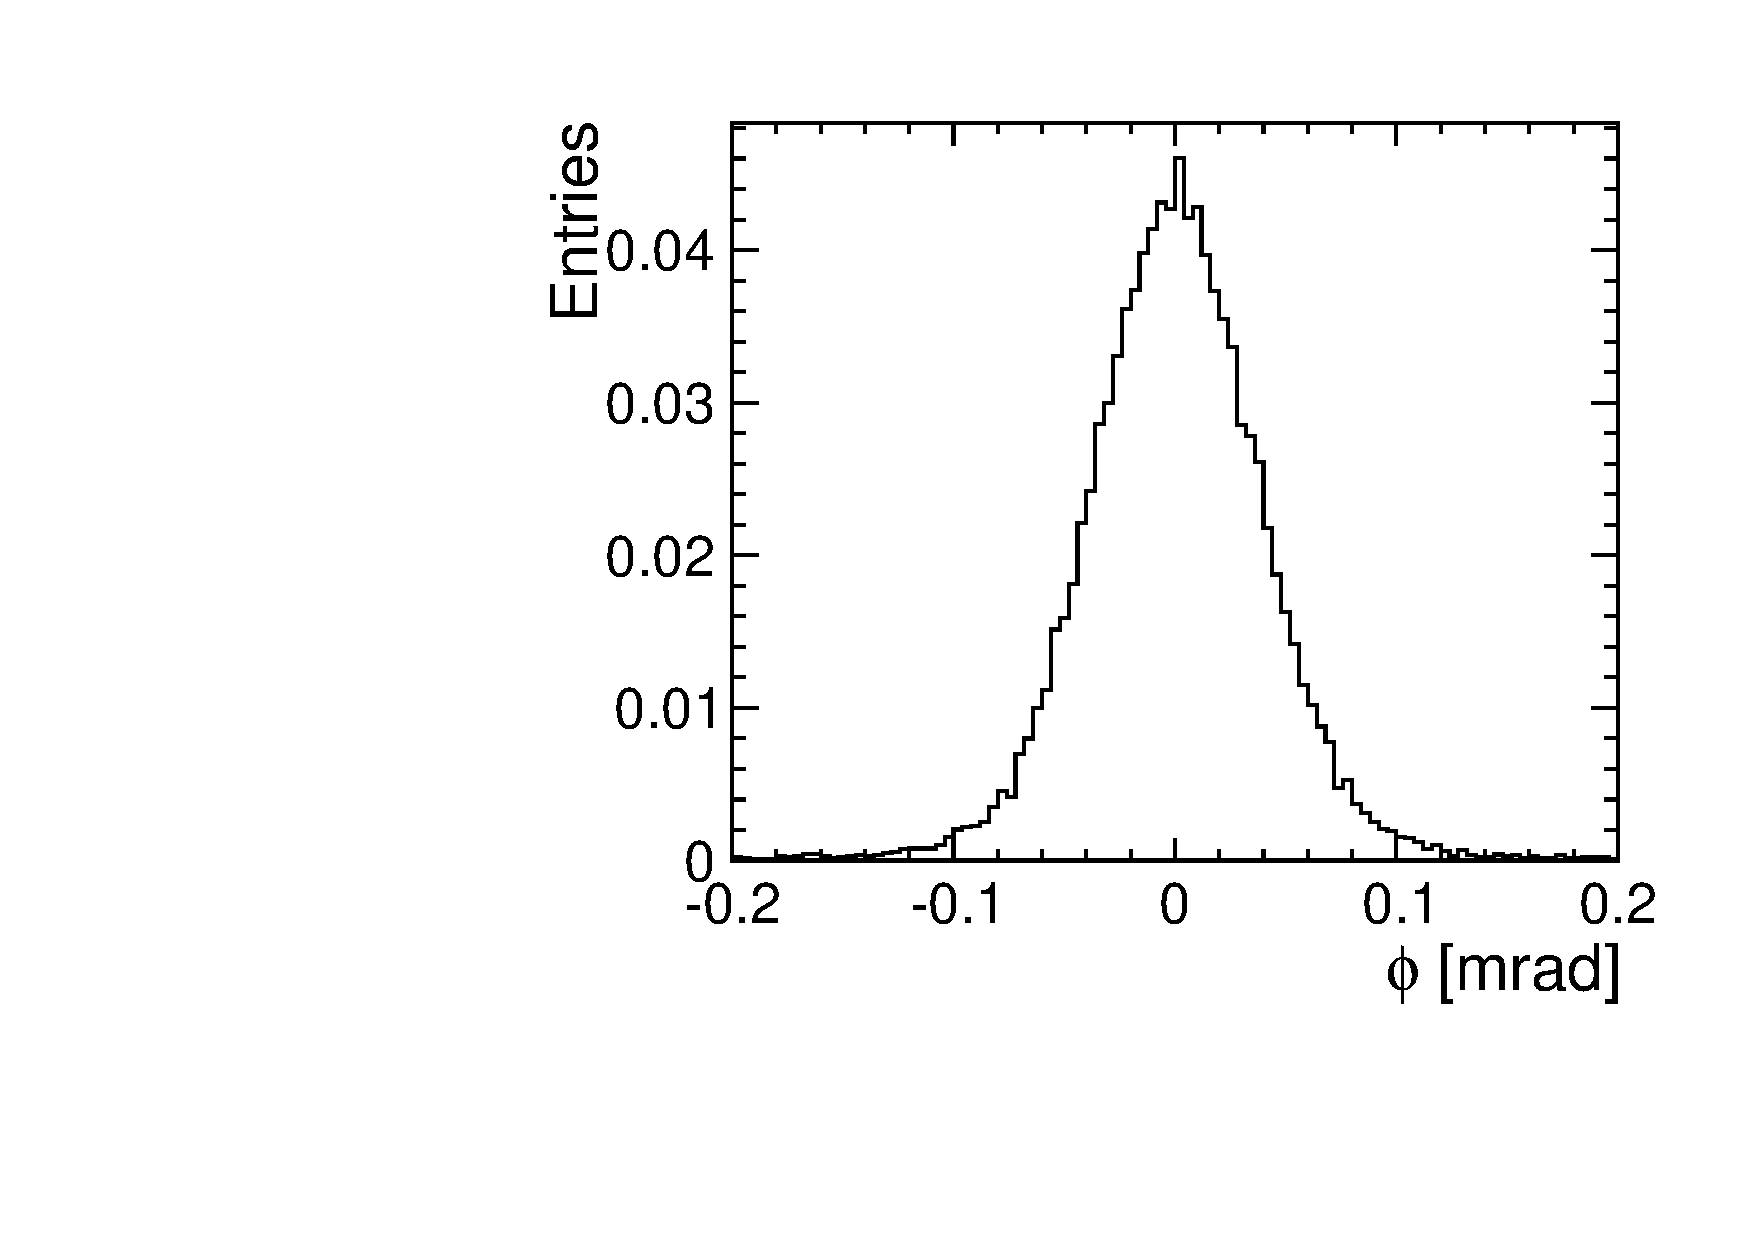
\includegraphics[width=\textwidth]{./figures/Telescope/MC_trackAnglePhi_planes_302_50.pdf}
    \caption{Track angle in $\phi$ (in horizontal direction)}
  \end{subfigure}\hfill
  \begin{subfigure}[b]{0.45\textwidth}
    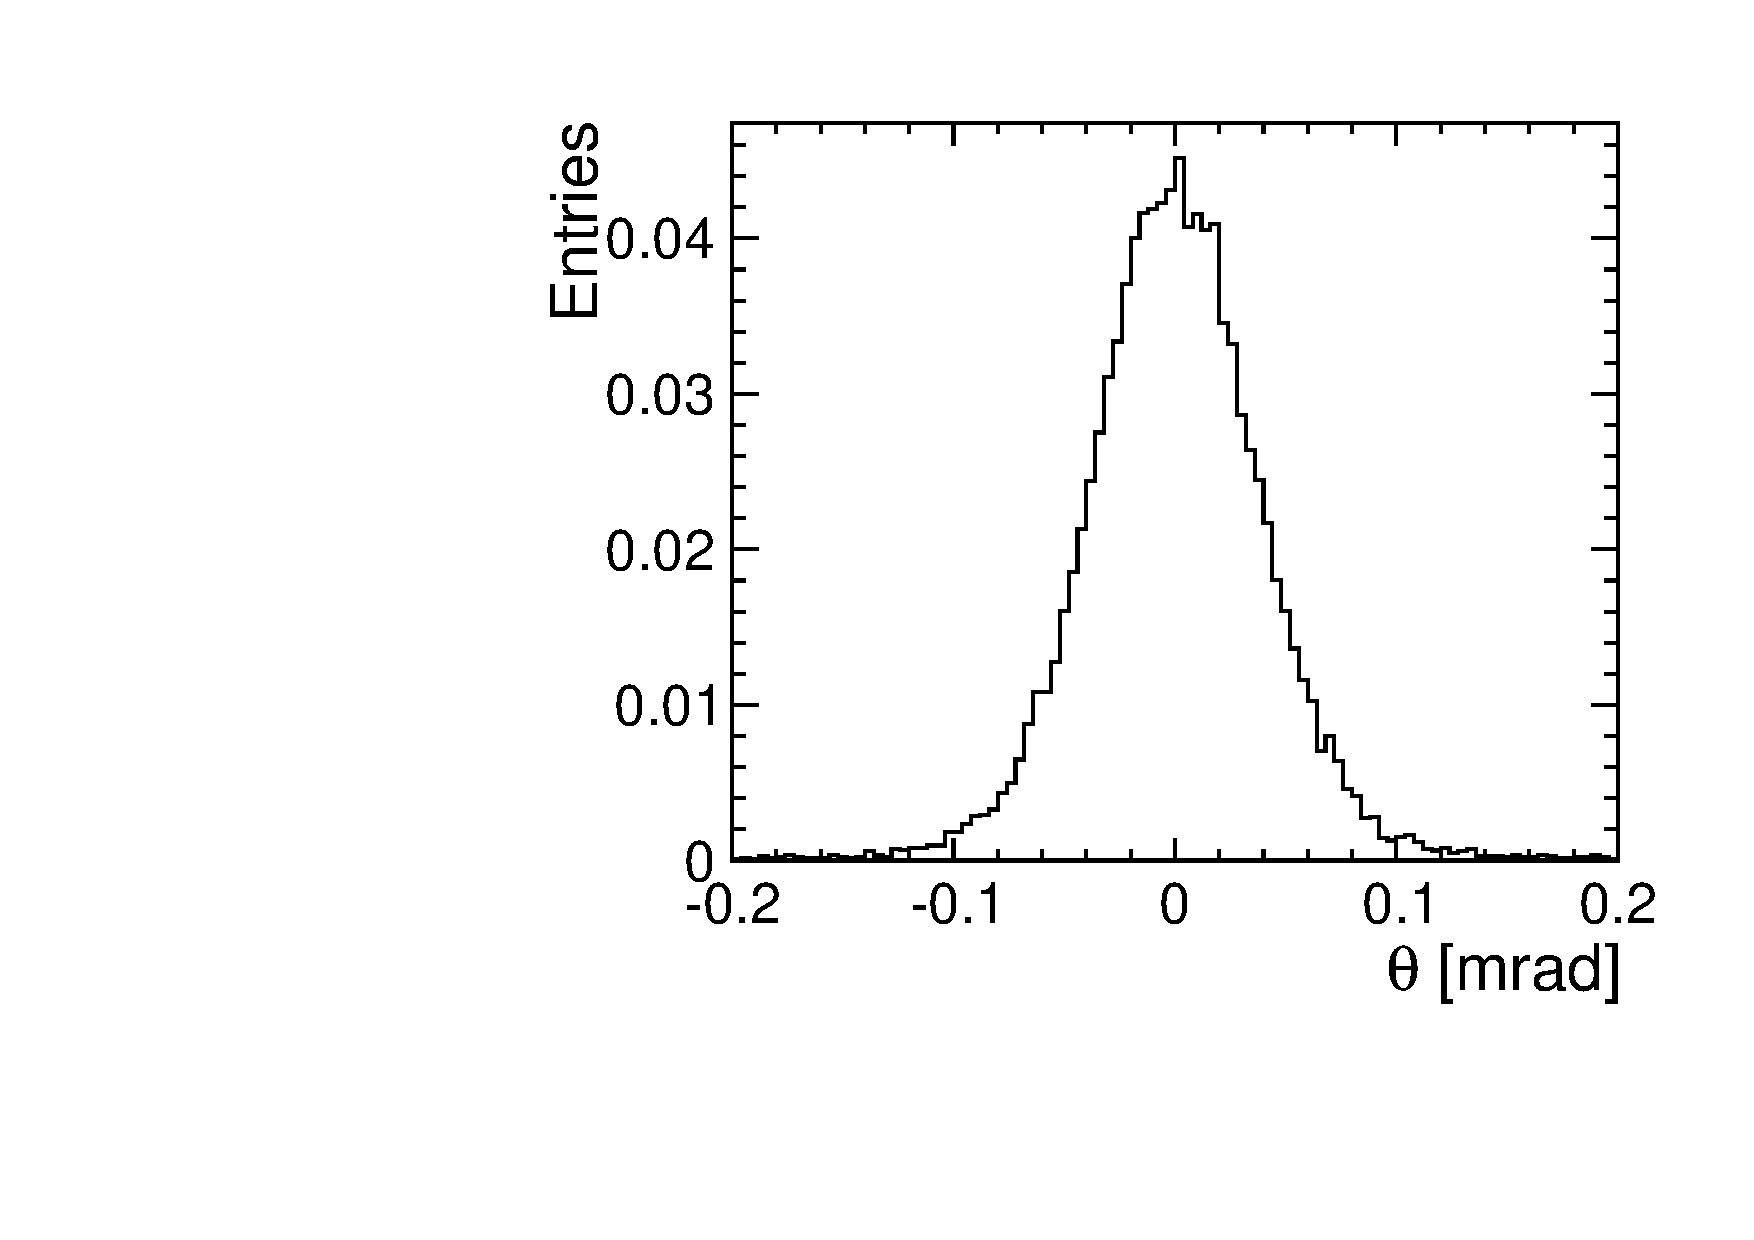
\includegraphics[width=\textwidth]{./figures/Telescope/MC_trackAngleTheta_planes_302_50.pdf}
    \caption{Track angle in $\theta$ (in vertical direction)}
  \end{subfigure}
  \caption{Track angular distribution in \textsc{Geant4} simulations
    due to multiple scatterings between the telescope plane 2 and the
    DUT obtained by comparing the global MC positions on the both
    planes.}
  \label{fig:MCbeamAngleDistr}
\end{figure}

The EUTelescope software framework (c.f. \cref{sec:EUTelescope}) is
used to reconstruct the hits on the telescope planes using the
$\eta$-correction method~\cite{Belau:1983eh}. The tracks are fitted
based on a $\chi^2$-minimisation method as described in
\cref{sec:EUTelescope}.

%% --------------------------------------------- %%
\subsection{Single-hit resolution on the telescope planes}

The bias and the depletion voltages, the sensor type and the threshold
values are the parameters defining the charge sharing and the cluster
size distribution. Therefore they define the intrinsic resolution of
the sensors.

% \begin{table}[htbp]
%   \centering
%   \caption{Parameters used for the simulation of the telescope planes in AllPix.}
%   \label{tab:AllPixTelescopePlanesParams}
%   \begin{tabular}{cccc}
%     \toprule
%     Bias voltage [V] & Depletion voltage [V] & Sensor type & Threshold [e-] \\
%     \midrule
%     50 & 30 & p-in-n & 1000 \\
%     \bottomrule
%   \end{tabular}
% \end{table}


\cref{fig:TelescopeCluSize_data_simu} compares the cluster size
distribution and the charge of the clusters in data and simulations
for the first telescope plane (plane 0). There is a good agreement
between the cluster-size distributions in data and simulations. The
small discrepancy might be due to the assumption on the un-calibrated
threshold value used in data which affects largely the cluster-size
distribution.

%% In
%% data, there are less single-pixel clusters due to slight imperfections
%% in the rotations of the planes while placing the telescope whereas the
%% simulation assumes a perfect placement of the telescope planes.

\begin{figure}[htbp] \centering
  \begin{subfigure}[b]{0.3\textwidth}
    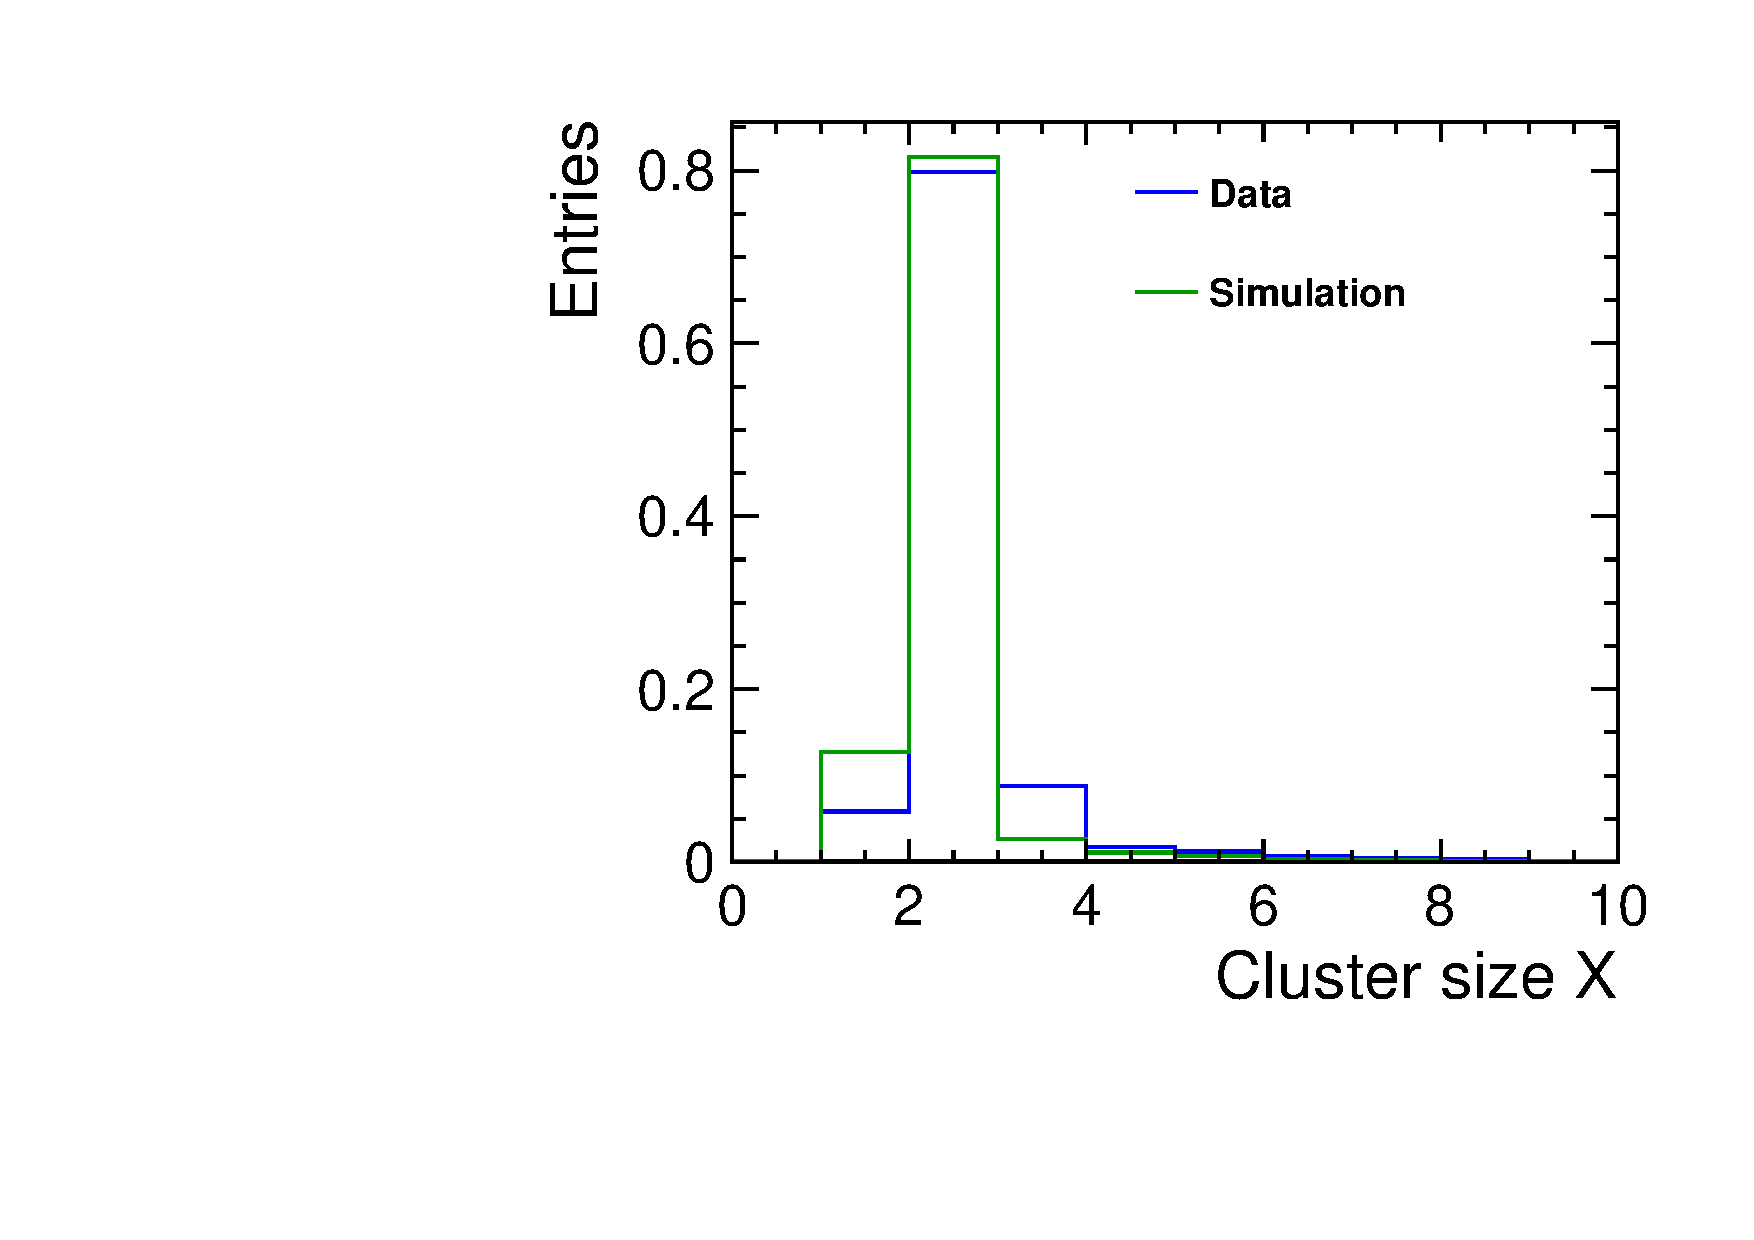
\includegraphics[width=\textwidth]{figures/Telescope/biasedResiduals/clusterSizeX_telescope0_data_simu.pdf}
    \caption{}
  \end{subfigure}\hfill
  \begin{subfigure}[b]{0.3\textwidth}
    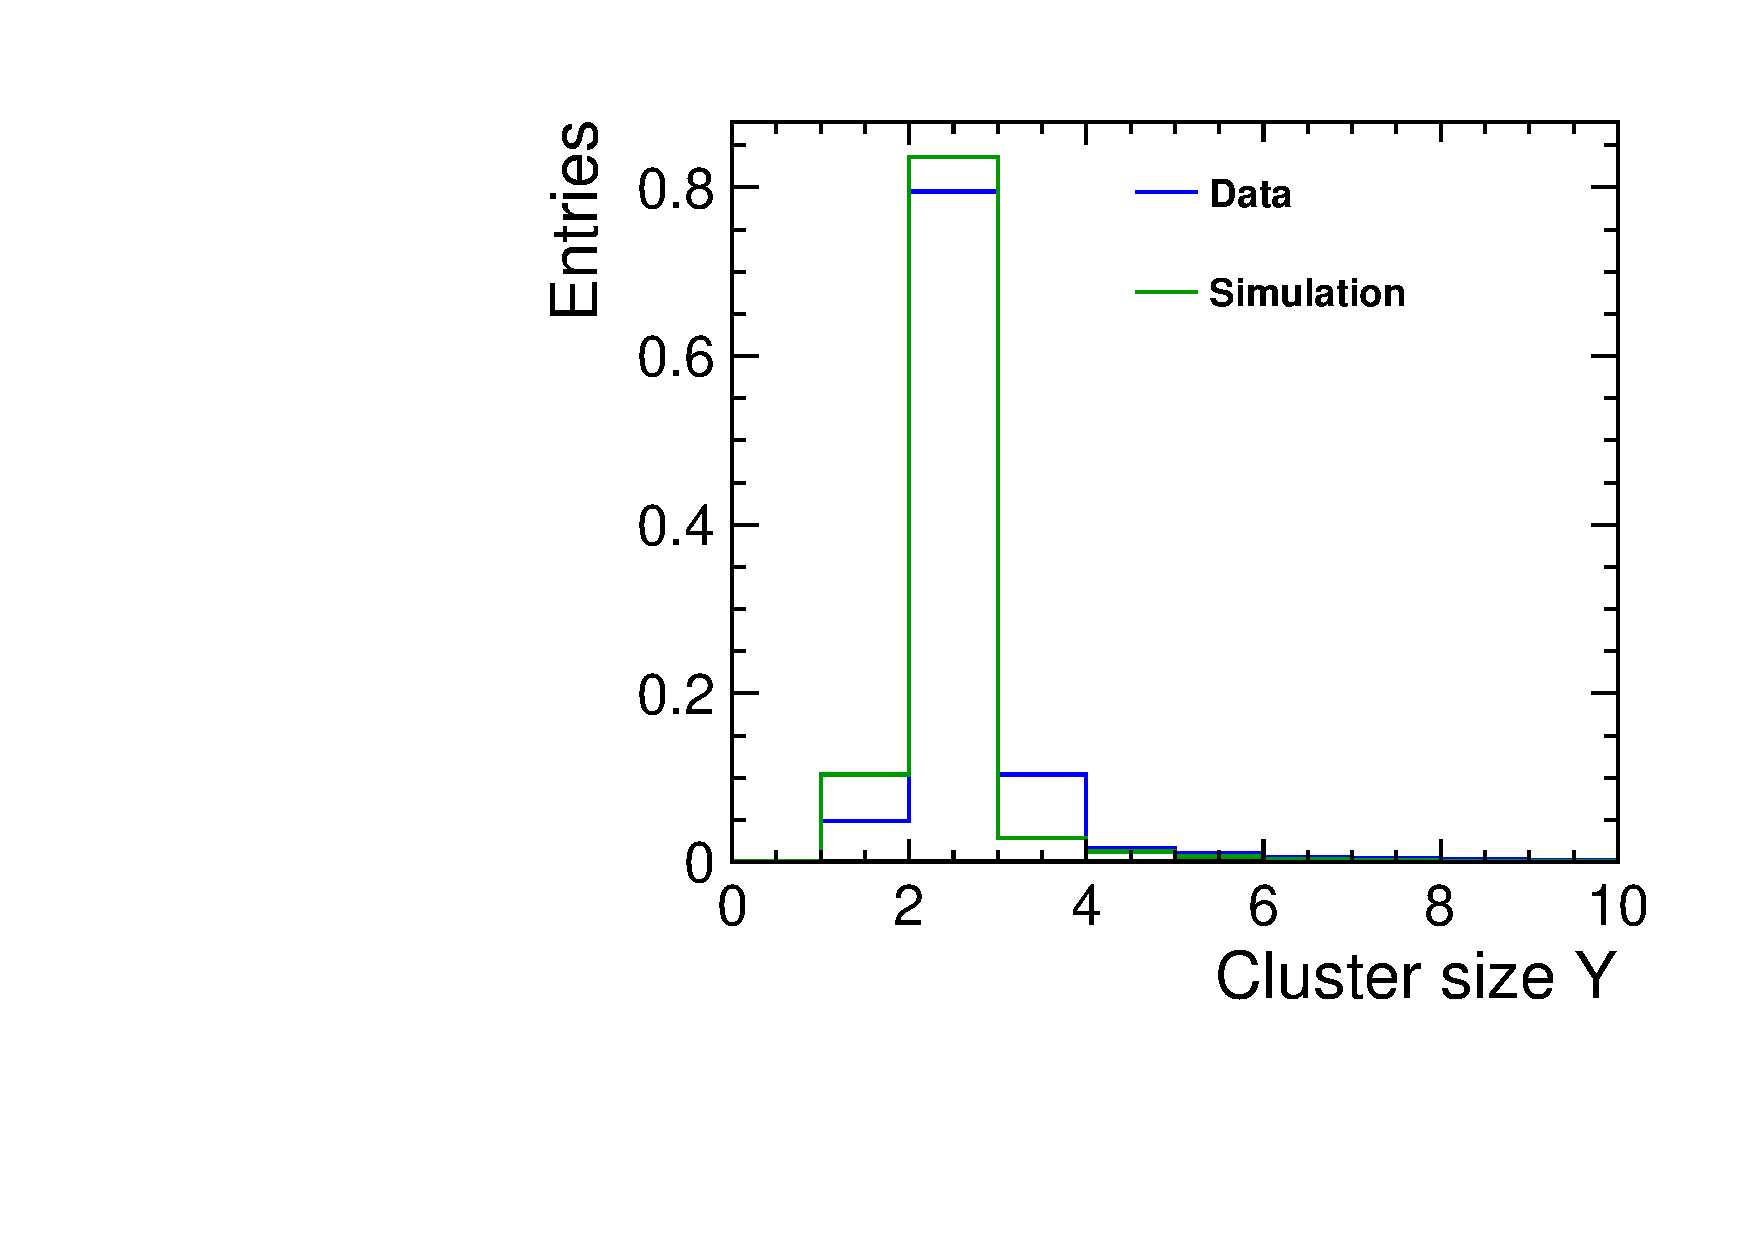
\includegraphics[width=\textwidth]{figures/Telescope/biasedResiduals/clusterSizeY_telescope0_data_simu.pdf}
    \caption{}
  \end{subfigure}\hfill
  \begin{subfigure}[b]{0.3\textwidth}
    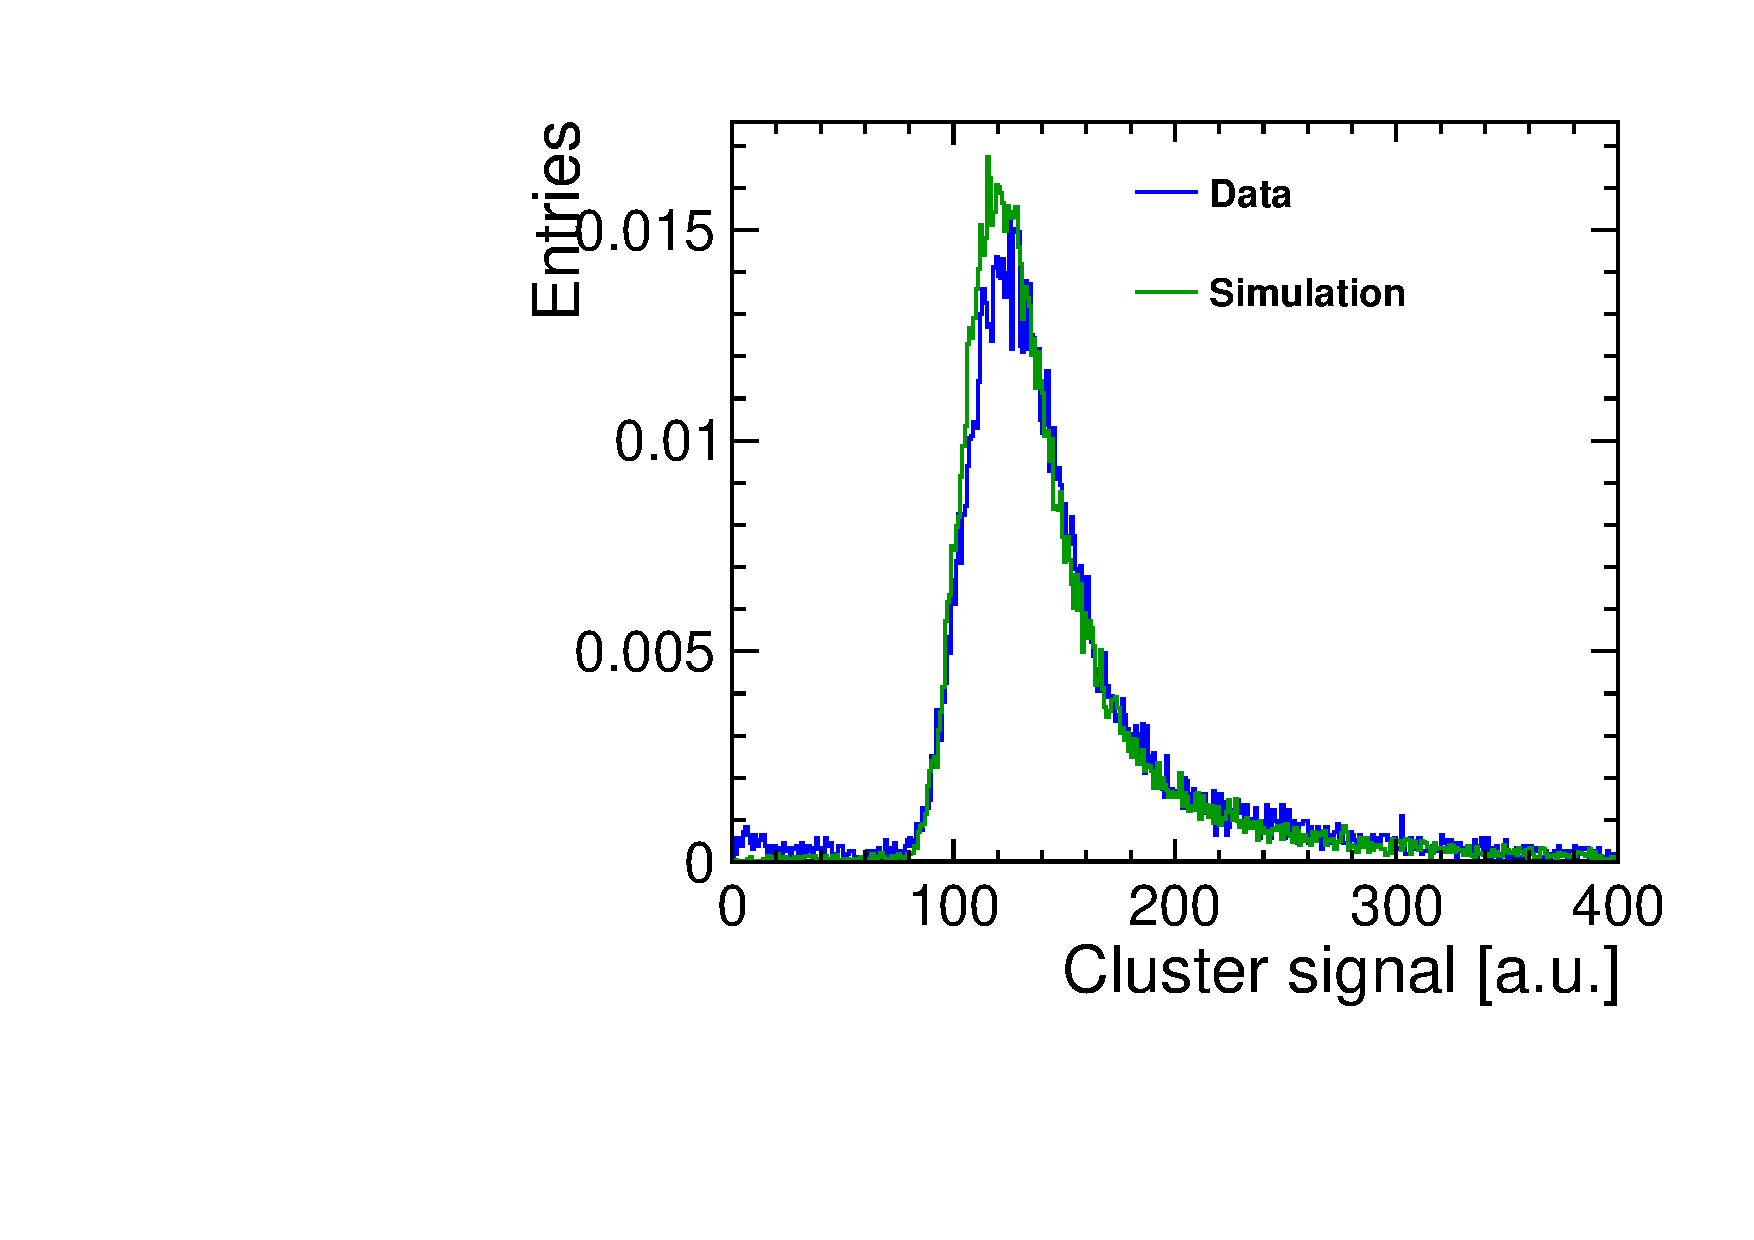
\includegraphics[width=\textwidth]{figures/Telescope/biasedResiduals/clusterSignal_telescope0_data_simu.pdf}
    \caption{}
  \end{subfigure}
  \caption{For the telescope plane 0, the cluster-size distribution in
    the (a) x direction and (b) y direction. (c) shows the sum of the
    charge in the cluster in units of
    TOT.} %data run 661, simulation run 54.
  \label{fig:TelescopeCluSize_data_simu}
\end{figure}

The hit resolution of a telescope plane is given by comparing the
reconstructed hit position with the Monte Carlo position
(x\textsubscript{MC} and y\textsubscript{MC}) obtained by AllPix
simulations. \cref{fig:TelPlane0_MC_hit} shows the hit residuals of
the first telescope plane in x and y directions in simulations. The
hit resolution is also considered as the intrinsic resolution of the
sensors. The standard deviation of a Gaussian fit to the center
$95.5\%$ of the residual distribution gives a resolution of
$\sim2.7\,\micron$. Since the residual distribution has a large tail,
the RMS of the distribution is higher ($\sim5.4\,\micron$). The tail
in the residuals distribution is due to the reconstruction of the hit
positions of single-pixel clusters where the charge sharing can not be
used to improved the reconstructed position.

% For this calculation, hits corresponding to tracks with the $10\%$ of
% highest $\chi^2$/NDF are ignored.

\begin{figure}[htbp] \centering
  \begin{subfigure}[b]{0.45\textwidth}
    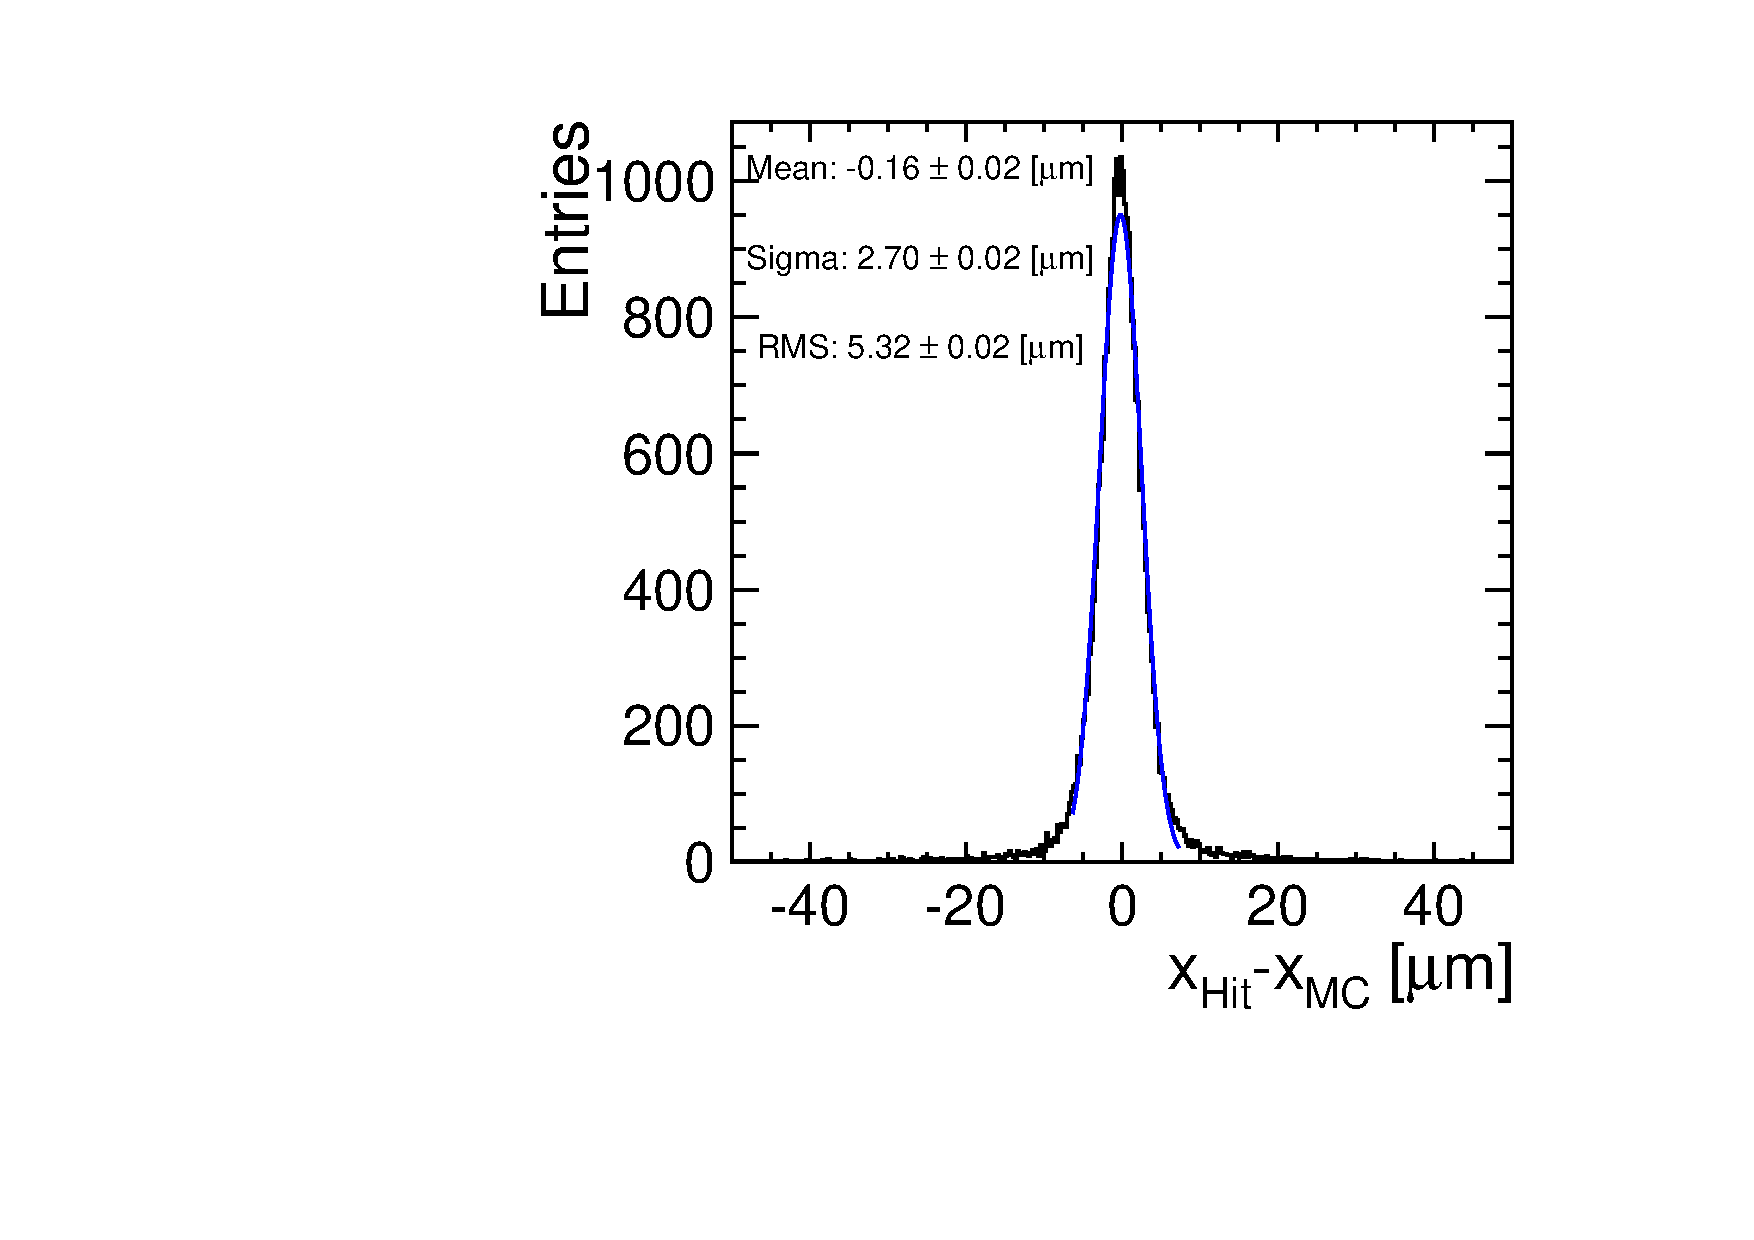
\includegraphics[width=\textwidth]{figures/Telescope/telescopePlane0_MC_vs_hit_x.pdf}
    \caption{}
  \end{subfigure}\hfill
  \begin{subfigure}[b]{0.45\textwidth}
    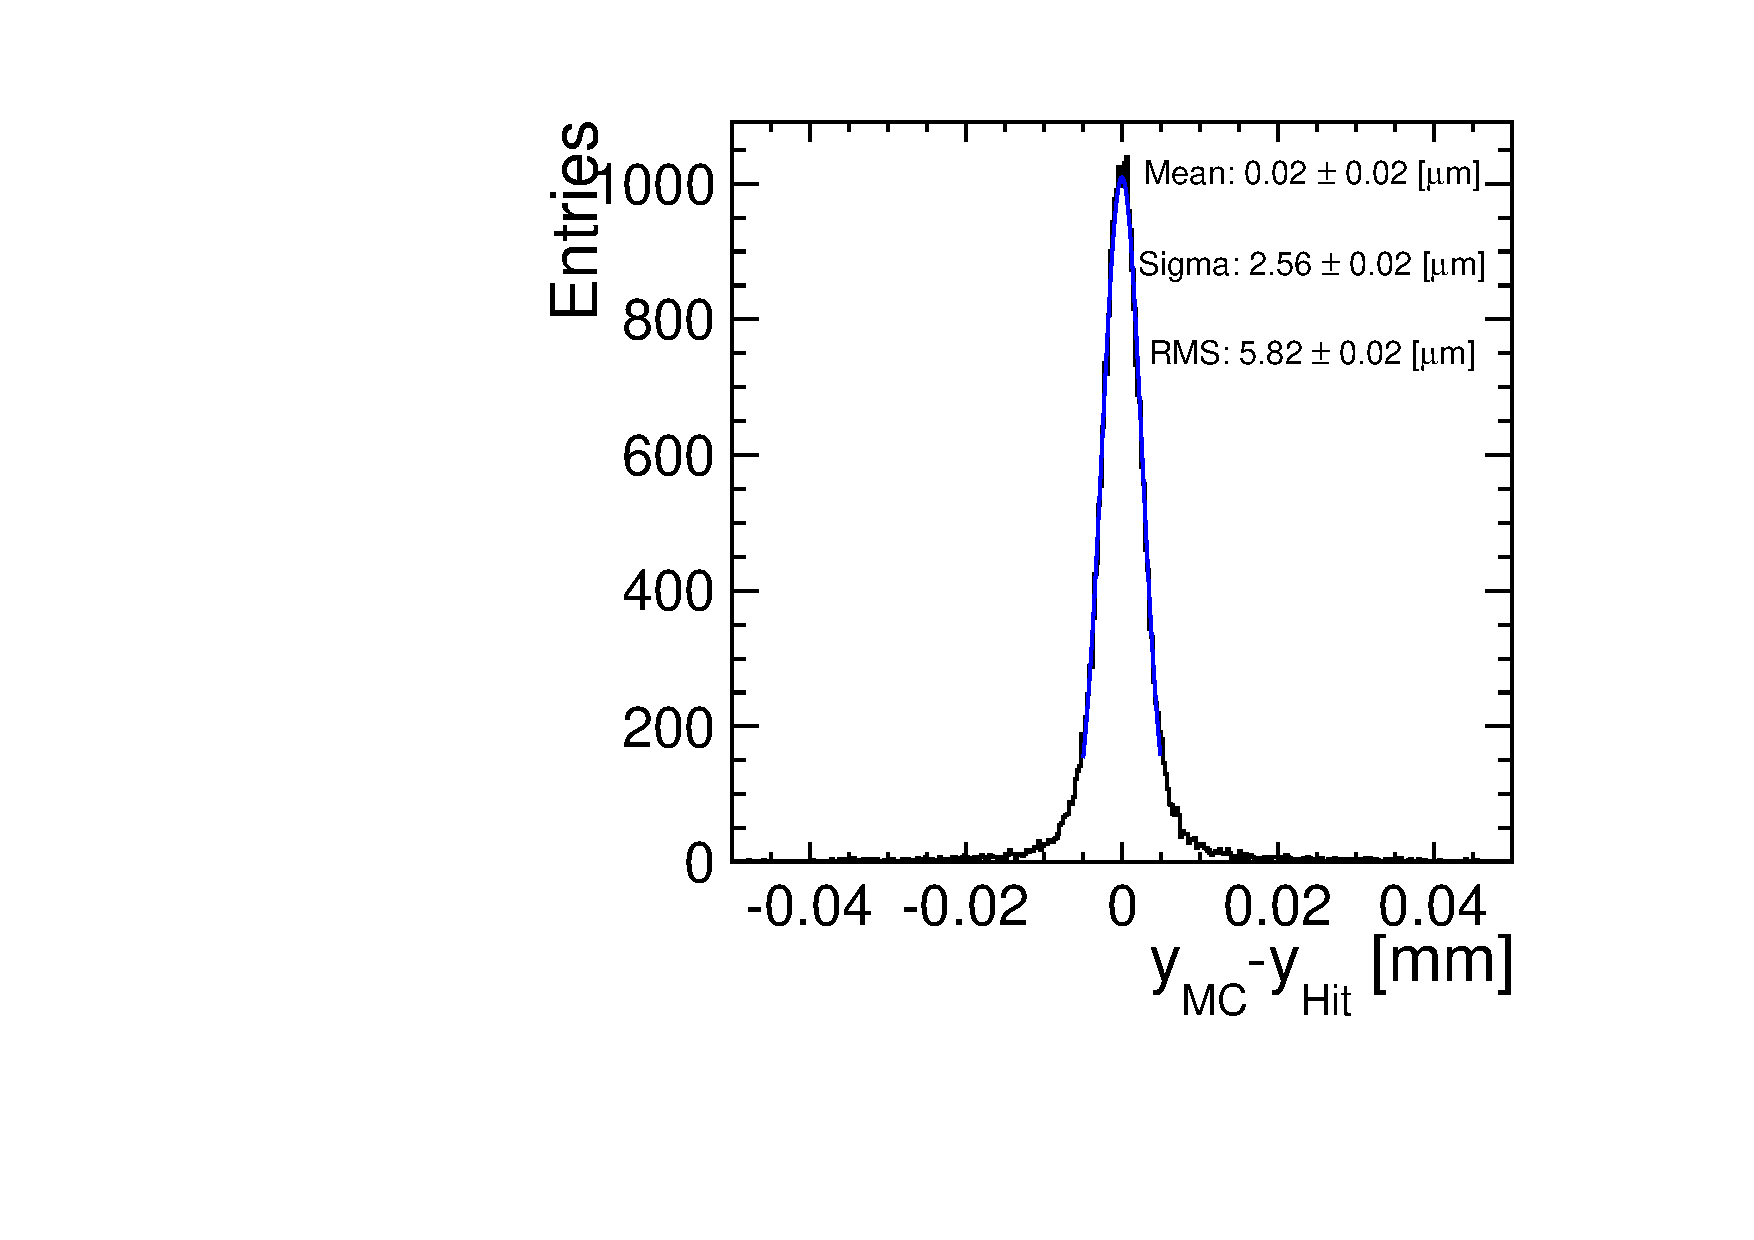
\includegraphics[width=\textwidth]{figures/Telescope/telescopePlane0_MC_vs_hit_y.pdf}
    \caption{}
  \end{subfigure}
  \caption{The hit residuals of a telescope plane in (a) x and (b) y
    directions given by comparing the MC and the reconstructed hit
    positions.}
  \label{fig:TelPlane0_MC_hit}
\end{figure}

The residuals for the first telescope plane as a function of the Monte
Carlo hit x\textsubscript{MC} and y\textsubscript{MC} are shown in
\cref{fig:TelPlane0_MC_hit_2D}. The intrinsic resolution does not
depend on the position of the hit. This confirms the coherence between
the geometry description in the AllPix simulations and the EUTelescope
reconstruction. The shape of these distributions is due to the beam
profile which is more focused in the middle of the sensors.

\begin{figure}[htbp] \centering
  \begin{subfigure}[b]{0.45\textwidth}
    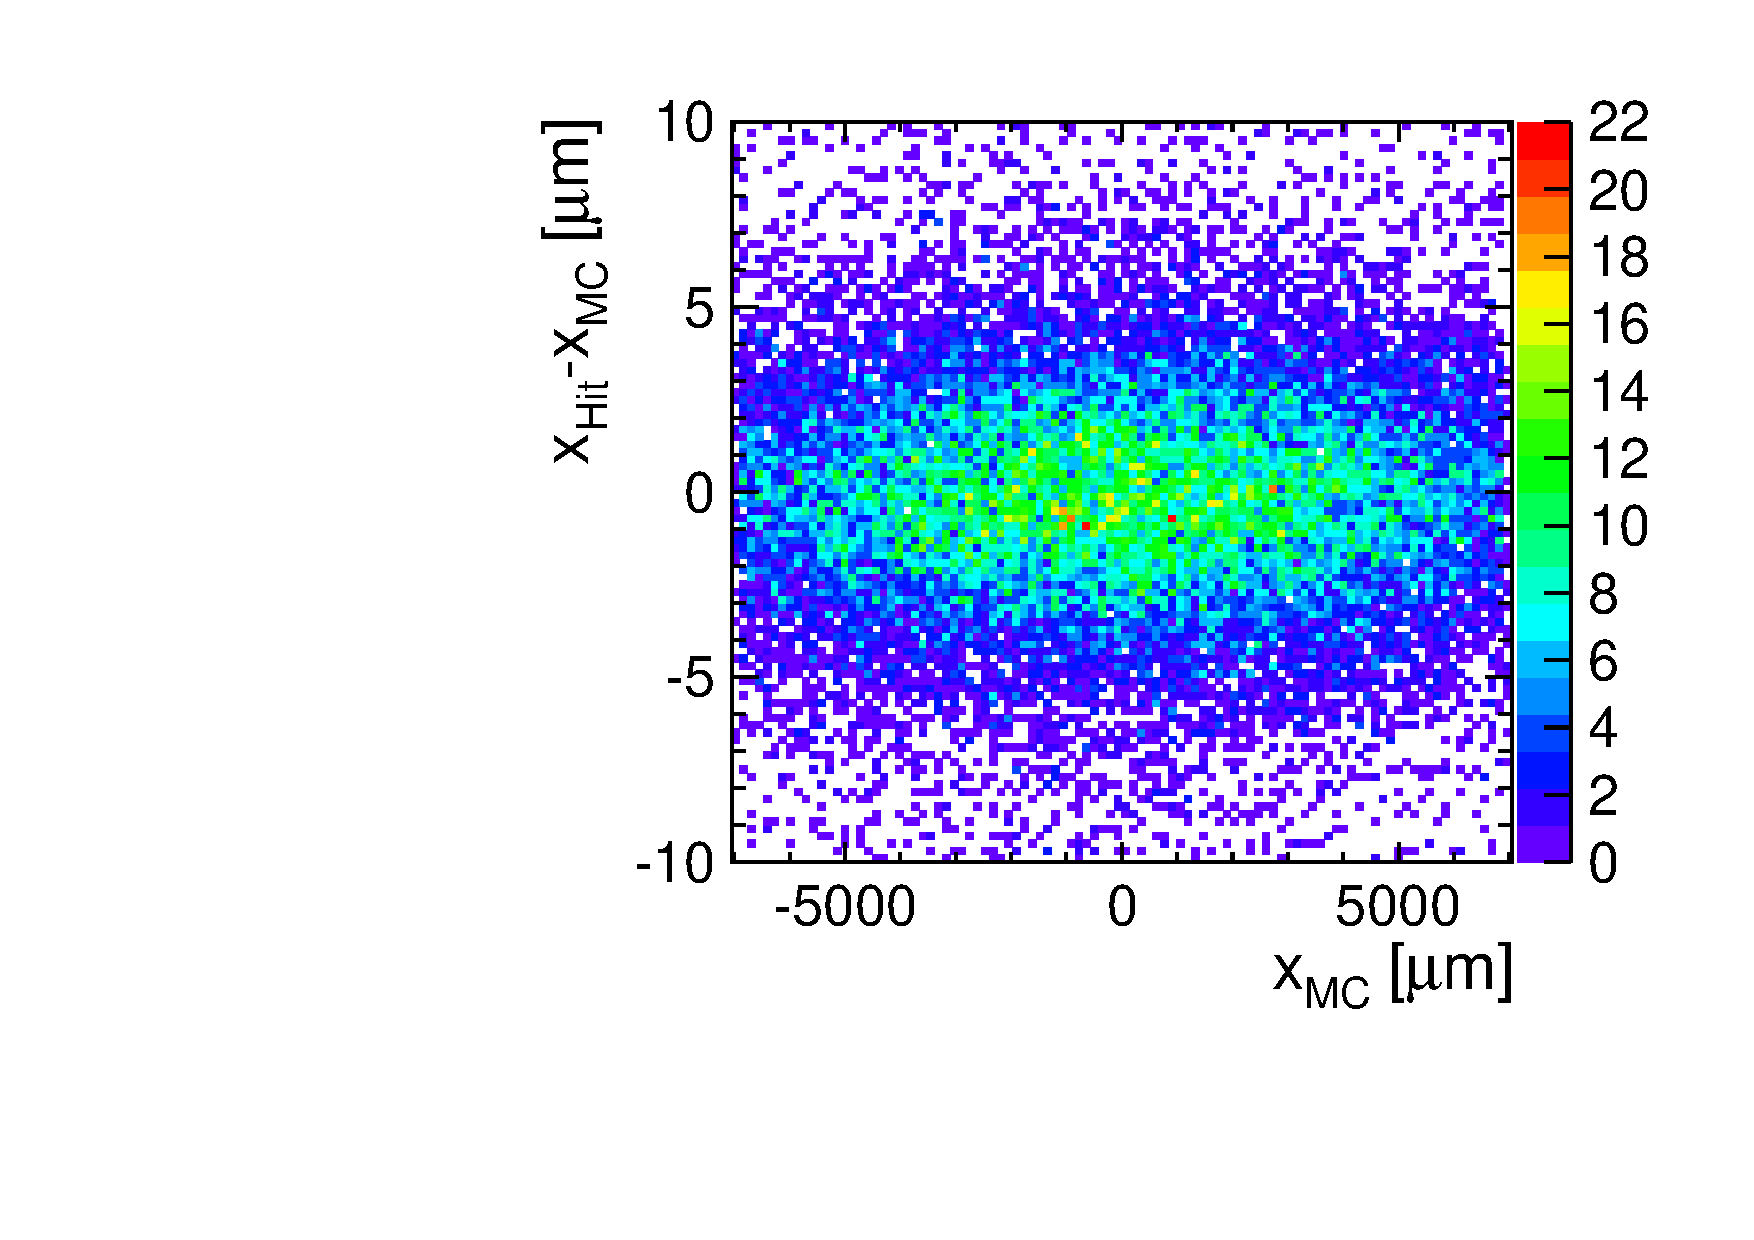
\includegraphics[width=\textwidth]{figures/Telescope/telescopePlane0_MC_vs_hit_x_2D.pdf}
    \caption{}
  \end{subfigure}\hfill
  \begin{subfigure}[b]{0.45\textwidth}
    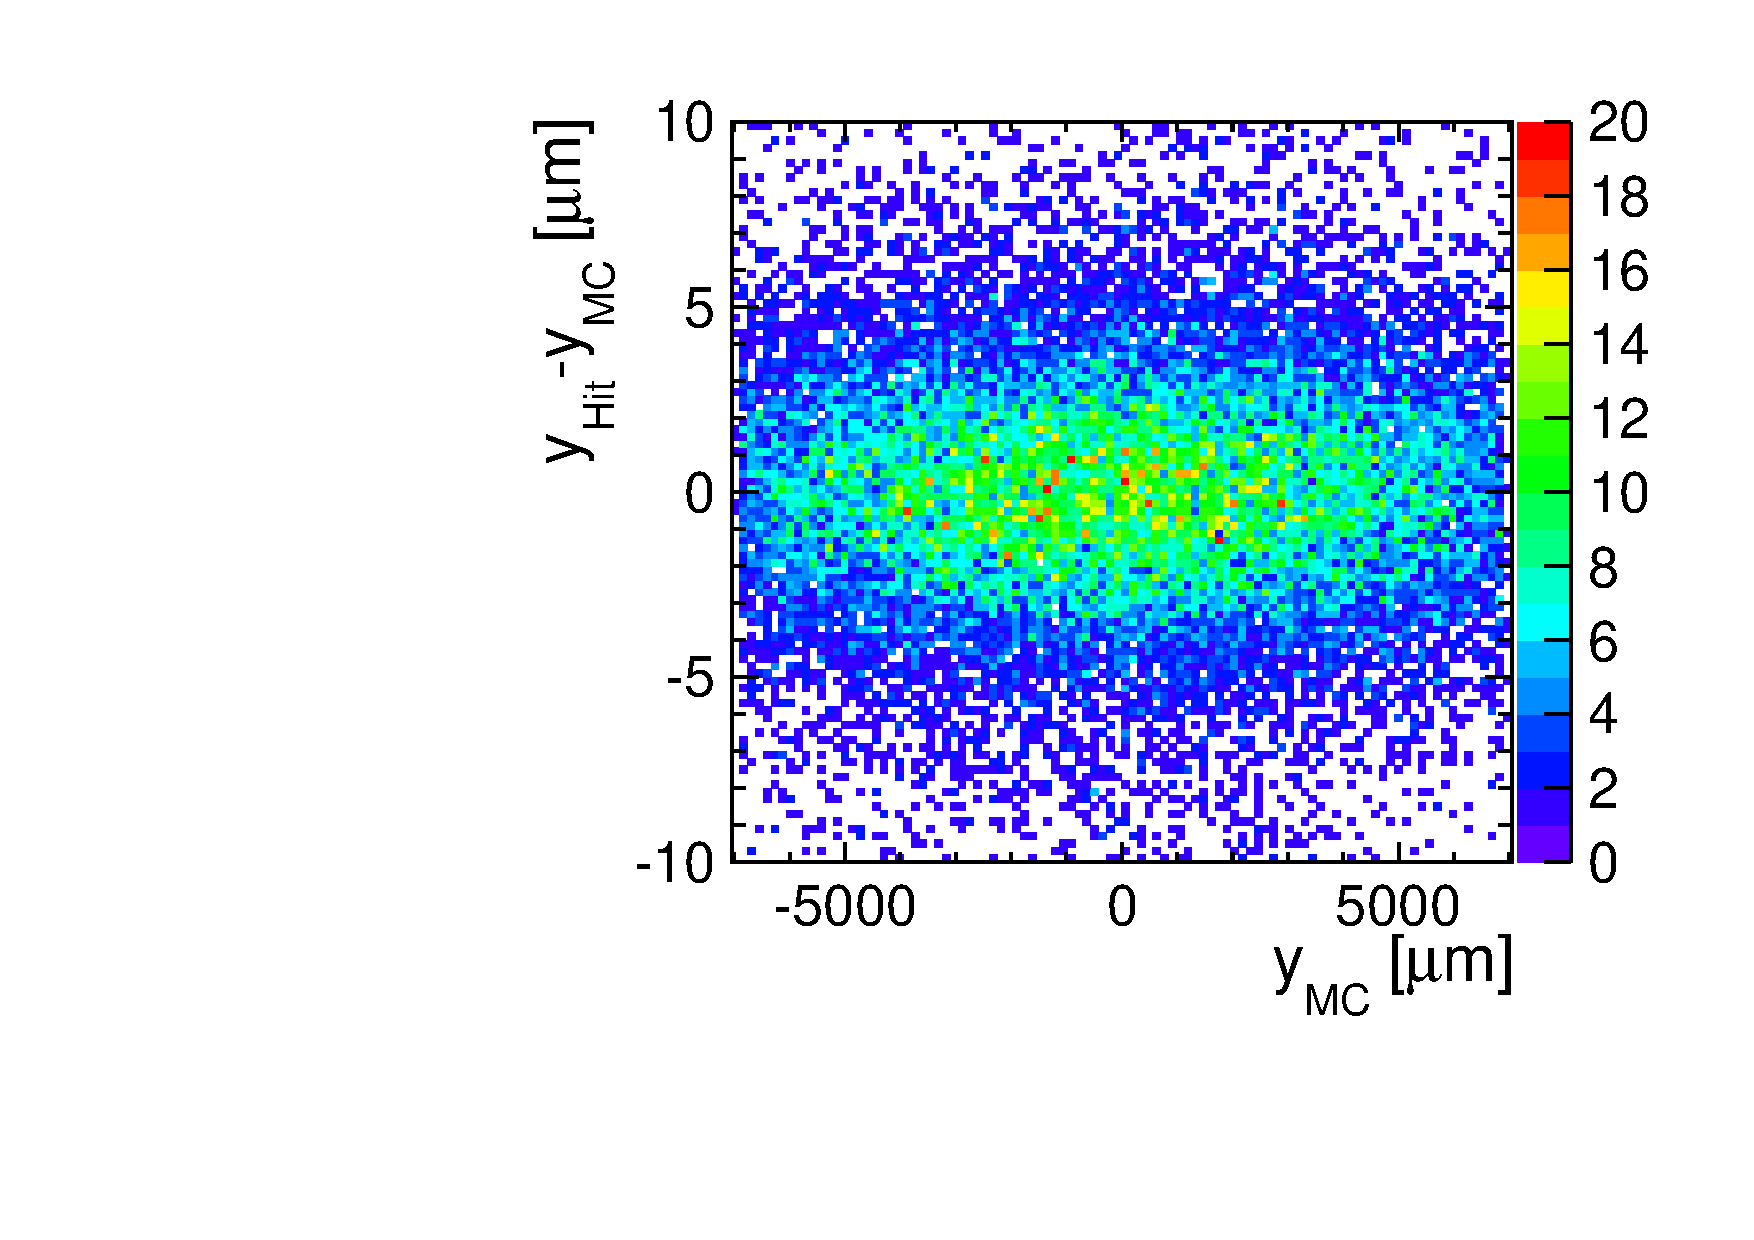
\includegraphics[width=\textwidth]{figures/Telescope/telescopePlane0_MC_vs_hit_y_2D.pdf}
    \caption{}
  \end{subfigure}
  \caption{The hit residuals of the first telescope plane in (a) x and
    (b) y directions comparing the MC and the reconstructed hit
    positions as a function of the MC position.}
  \label{fig:TelPlane0_MC_hit_2D}
\end{figure}


%% --------------------------------------------- %%
\subsection{Biased residuals on each telescope plane}

The tracks on the telescope planes are reconstructed using a
$\chi^2$-minimisation method as described in
\cref{sec:EUTelescope}. The biased residual on each telescope plane is
defined as the difference between the measured hit and the fitted
track position. It determines the precision with which the track is
reconstructed and depends on the hit resolution of the telescope
sensors, the number of measurements and their positions and on the
amount of multiple scattering. The residual is biased because the
track fit includes the telescope plane of the measured hit.

The biased residual width $r_b^2(z)$, for tracks at all positions
$z=z_i$ at the telescope planes, can be expressed
as~\cite{Jansen:2016bkd}:

\begin{equation}
r_b^2(z)=\sigma_{int}^2(z)-\sigma_{t,b}^2(z) \; , 
\end{equation}

where $\sigma_{int}$ is the intrinsic hit resolution of the sensors
and $\sigma_{t,b}$ is the biased track resolution. $\sigma_{t,b}$
determines the precision with which the particle trajectory is defined
with a biased track. For the inner planes of the telescope, since more
measurement points contribute to the track reconstruction,
$\sigma_{t,b}$ decreases which leads to higher values for the biased
residuals. Whereas, for the outer planes where less measurement points
contribute (planes 0 and 6), $\sigma_{t,b}$ gets worse (increases)
resulting in a narrower $r_b$ distribution.

The biased residuals depend highly on the quality of the tracks. The
tracks with high $\chi^2$/NDF go through more multiple scatterings and
therefore contribute to the tails of the biased residuals. For the
in-pixel analysis done in \cref{ch:ThinSensorsStudies}, the tracks
with a $\chi^2$/NDF higher than 100 are discarded. This cut is applied
for all tracks used in this analysis.

\cref{fig:chi2_data_simu} shows the $\chi^2$/NDF distributions in data
(a) and in simulations (b) with the cut at 100 on the $\chi^2$/NDF as
illustrated with a red line.

\begin{figure}[htbp] \centering
  \begin{subfigure}[b]{0.45\textwidth}
    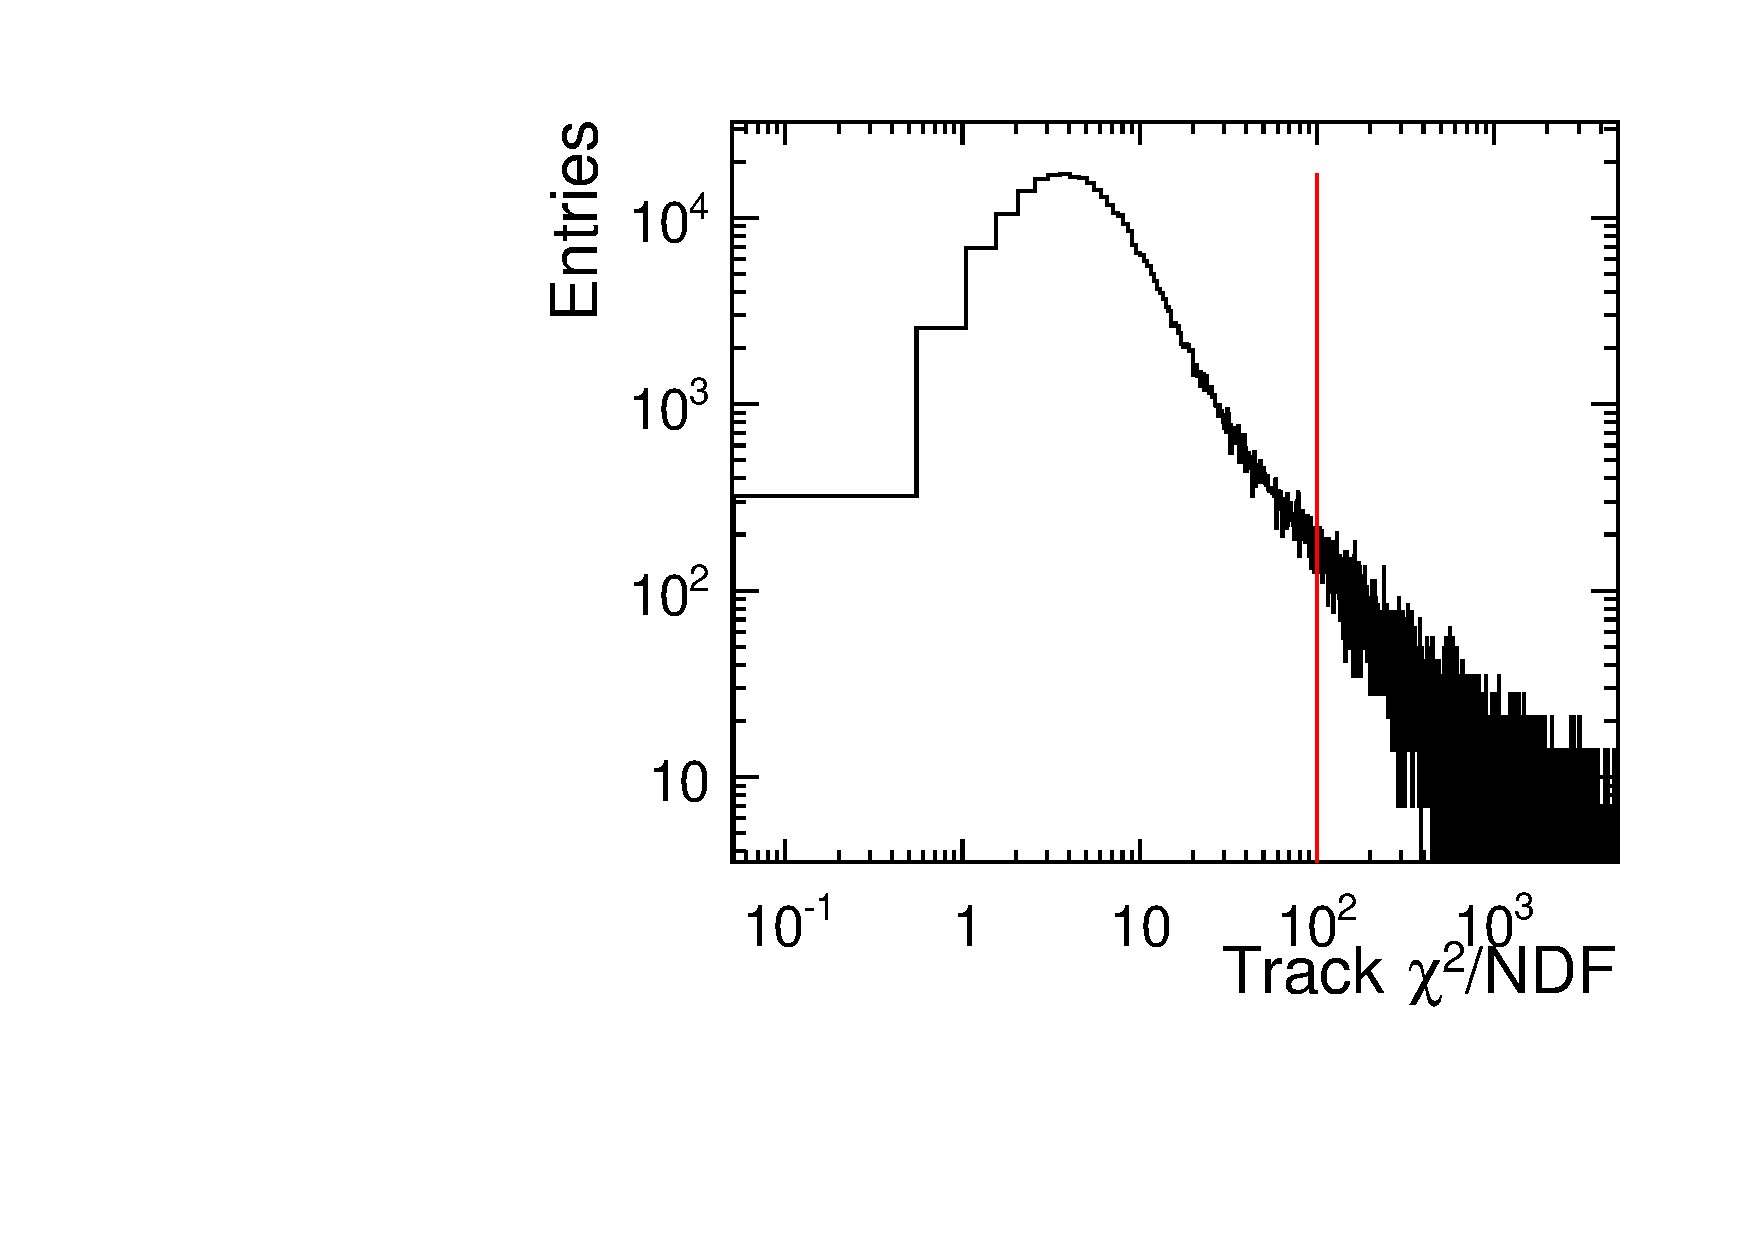
\includegraphics[width=\textwidth]{figures/Telescope/biasedResiduals/chi2_run661.pdf}
    \caption{Data}
  \end{subfigure}\hfill
  \begin{subfigure}[b]{0.45\textwidth}
    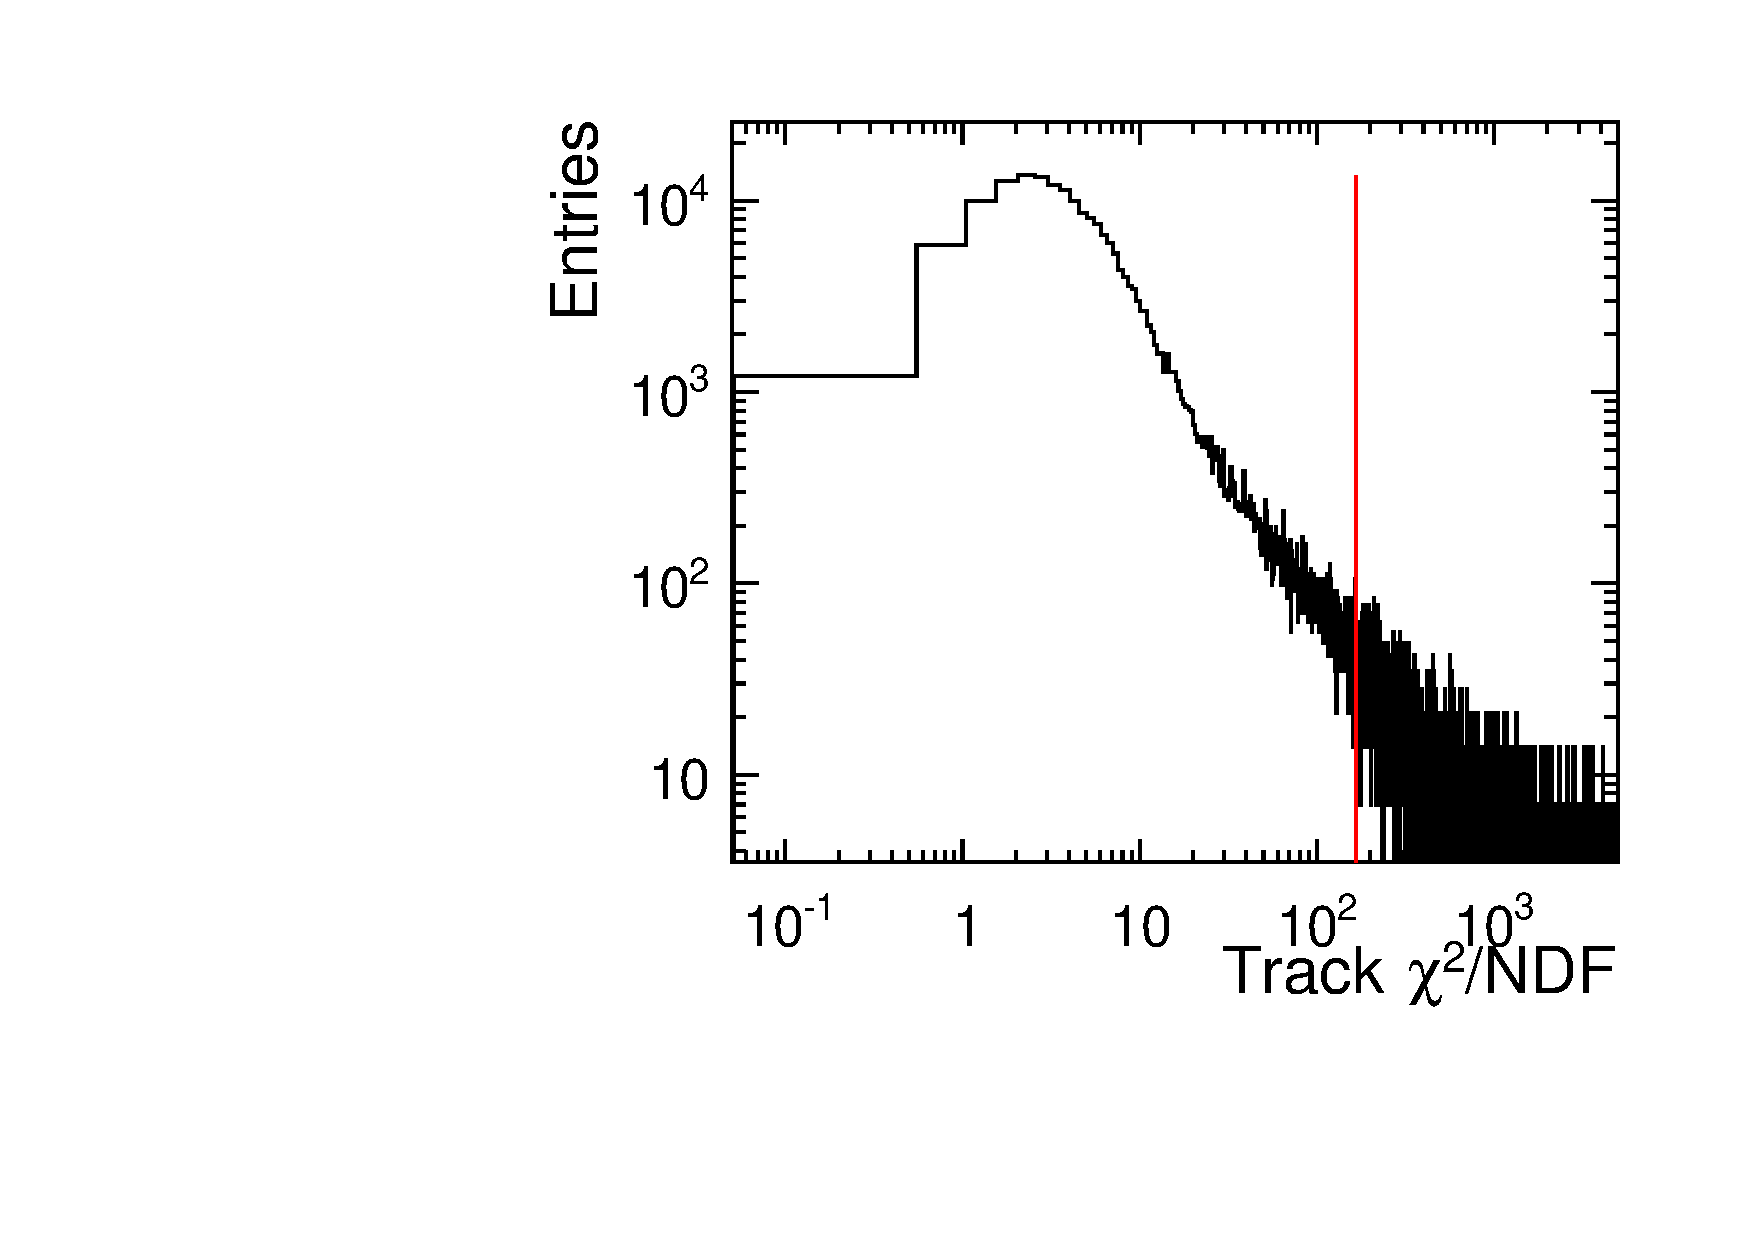
\includegraphics[width=\textwidth]{figures/Telescope/biasedResiduals/chi2_run77.pdf}
    \caption{Simulation}
  \end{subfigure}
  \caption{$\chi^2$/NDF distributions for reconstructed telescope
    tracks for (a) data and (b) simulation. A cut is applied to
    discard the tracks with $\chi^2$/NDF higher than 100 (illustrated
    with the red line).}
  \label{fig:chi2_data_simu}
\end{figure}

\cref{fig:telescopeBiasedRMS_data_simu} compares the RMS of the biased
residuals in data and simulations for a cut applied to discard the
tracks with $\chi^2$/NDF higher than 100. The residual distributions
are given in
\cref{fig:telescope_biasedResiduals_data_X,fig:telescope_biasedResiduals_data_Y}
for data and
\cref{fig:telescope_biasedResiduals_simu_X,fig:telescope_biasedResiduals_simu_Y}
for simulation.

\begin{figure}[htbp] \centering
  \begin{subfigure}[b]{0.45\textwidth}
    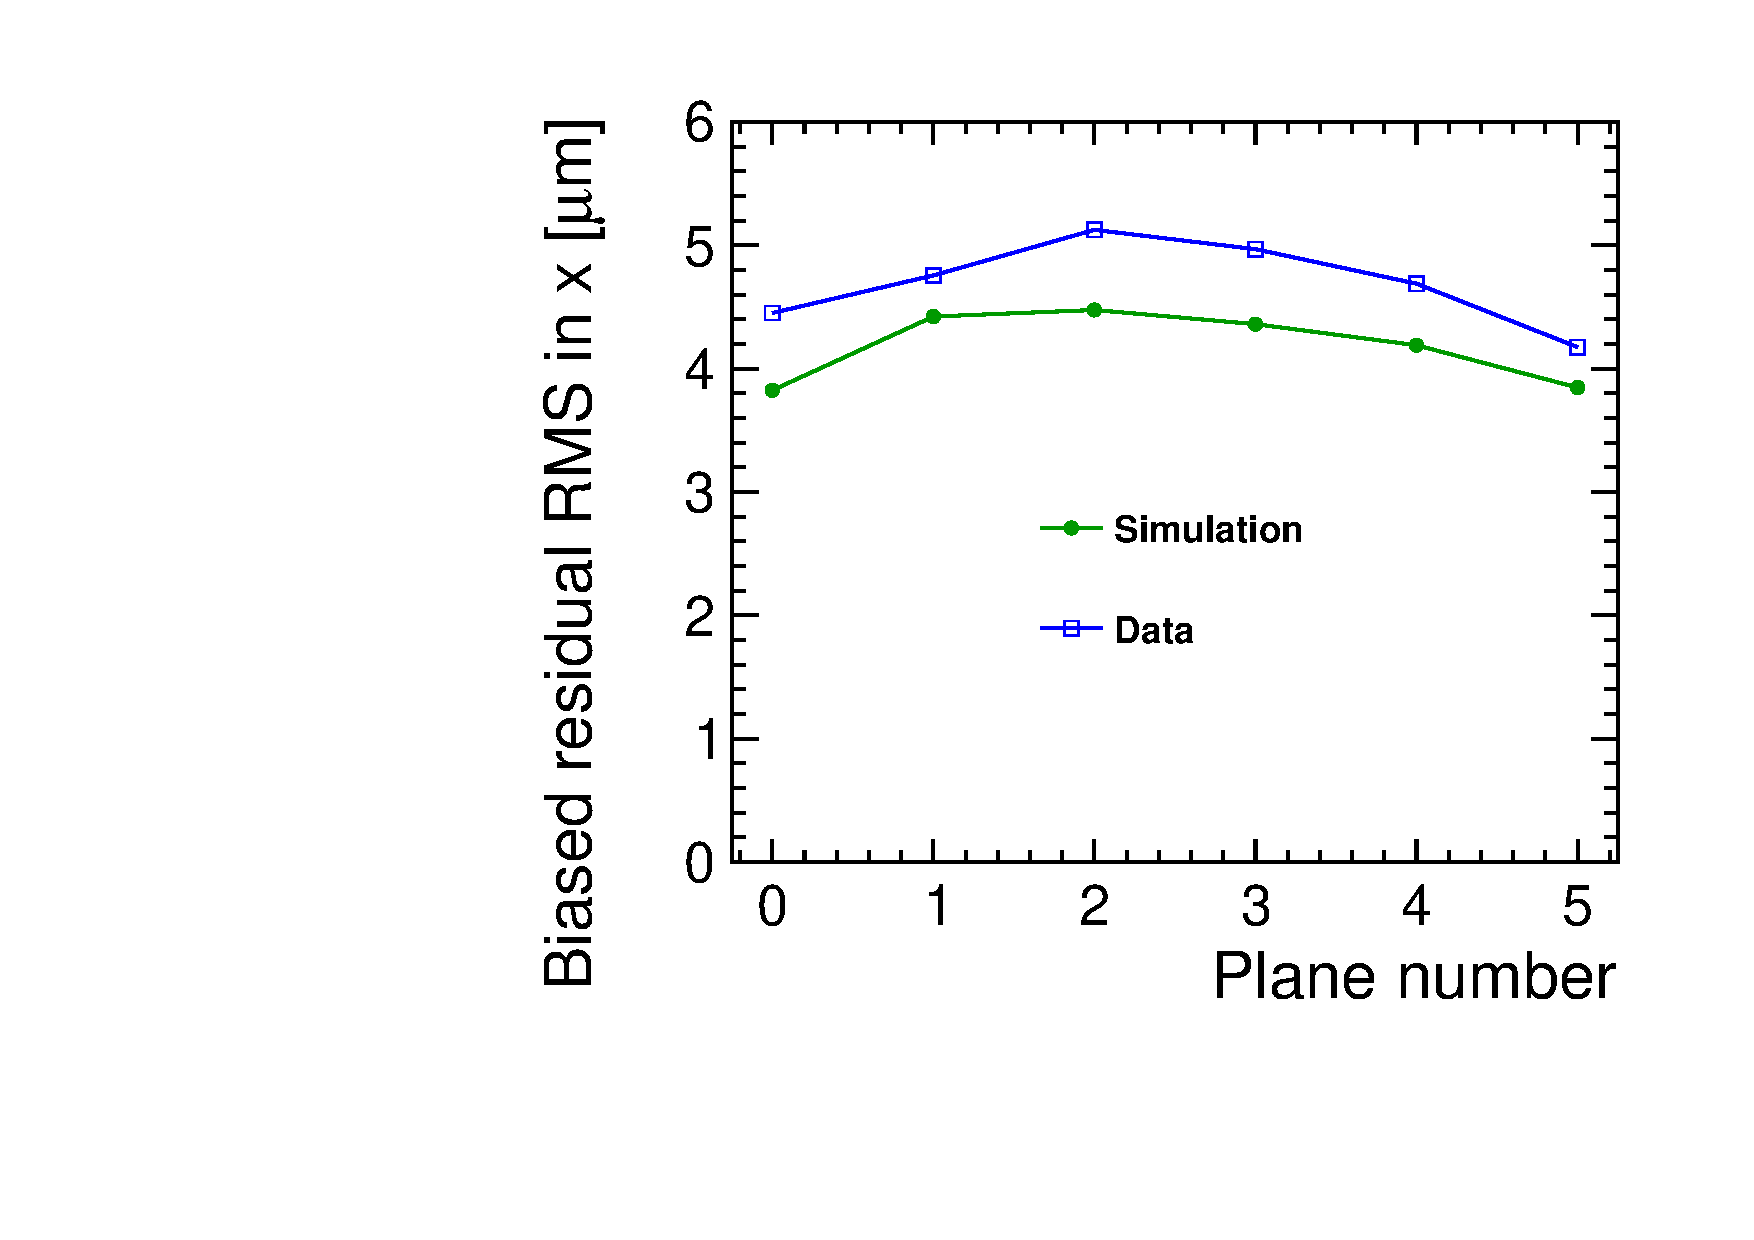
\includegraphics[width=\textwidth]{figures/Telescope/biasedResiduals/RMSX_simu_vs_data.pdf}
    \caption{}
  \end{subfigure}\hfill
  \begin{subfigure}[b]{0.45\textwidth}
    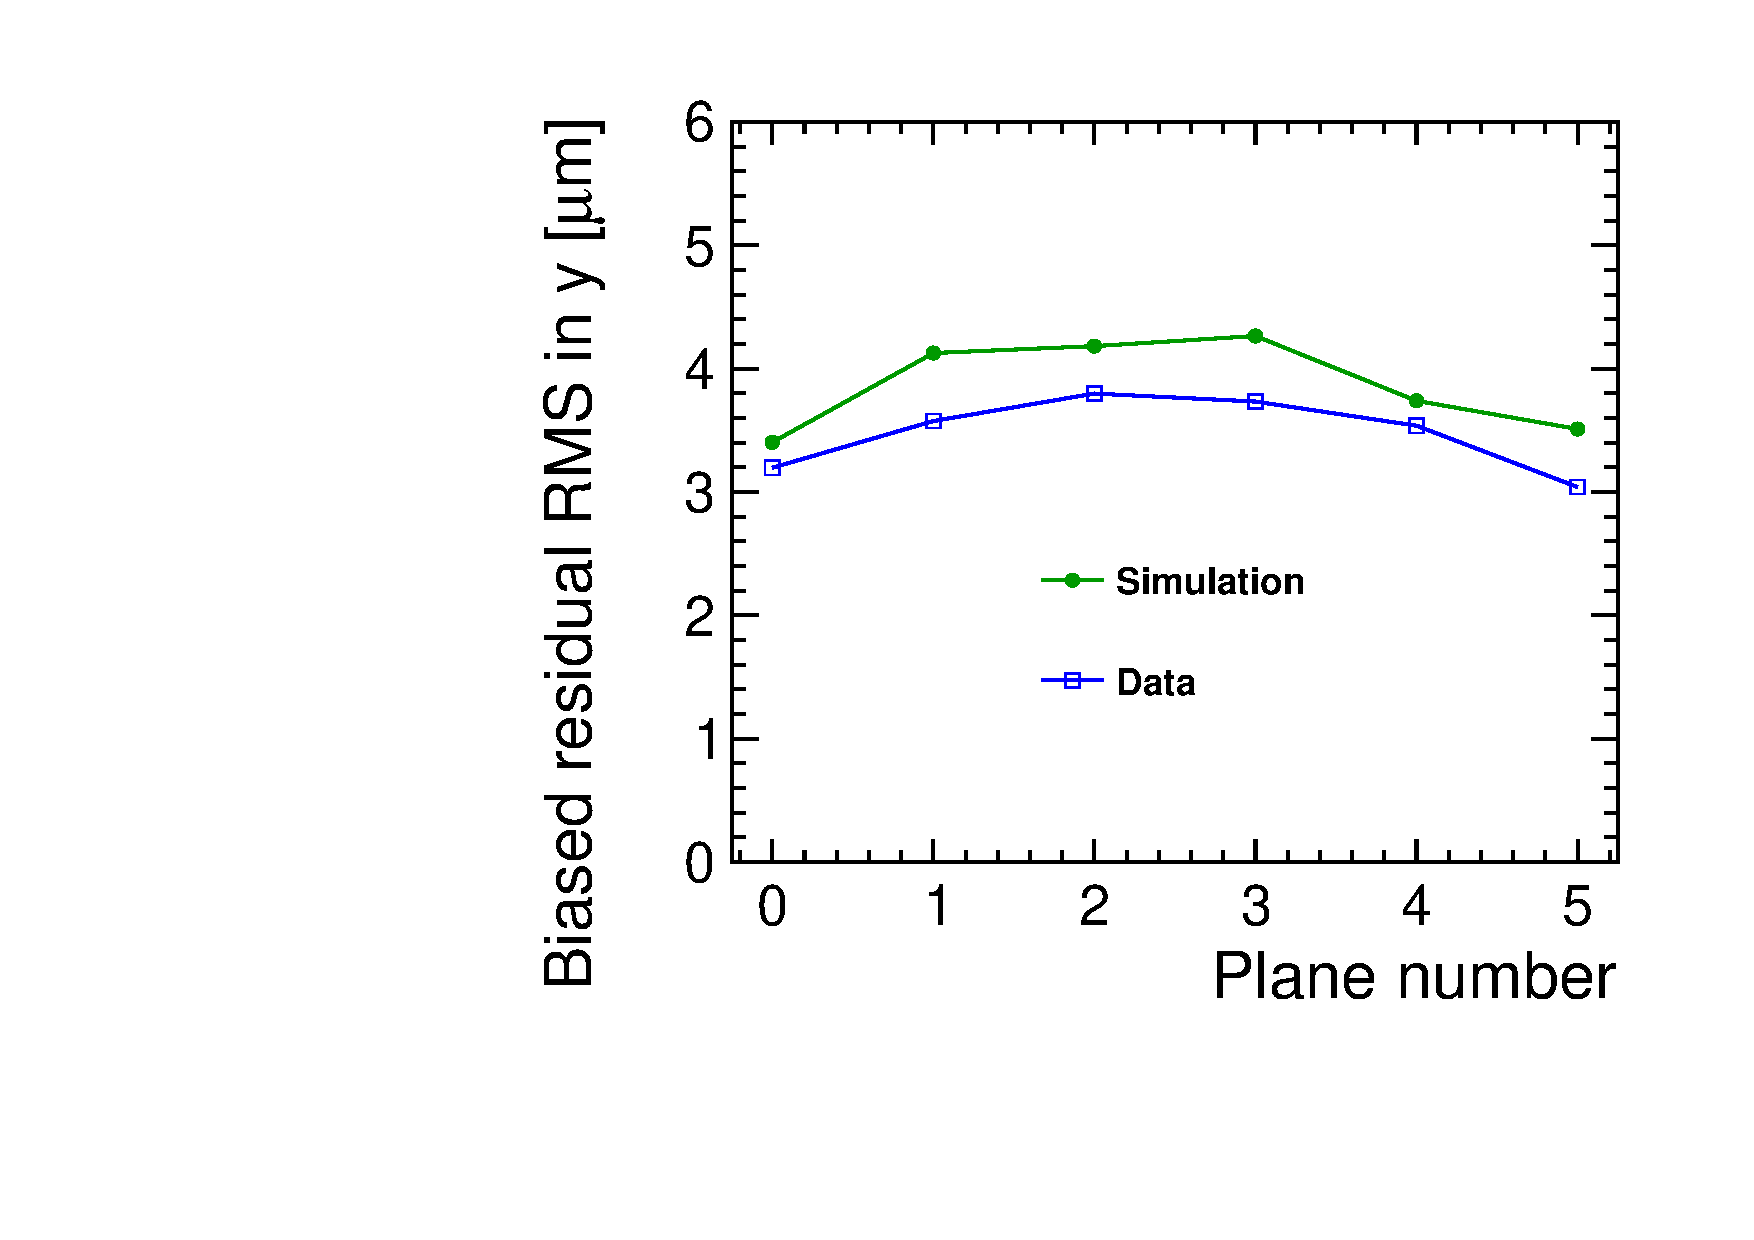
\includegraphics[width=\textwidth]{figures/Telescope/biasedResiduals/RMSY_simu_vs_data.pdf}
    \caption{}
  \end{subfigure}
  \caption{The RMS of the biased residuals $r_b$ in the (a) x and (b) y
    directions comparing the data and simulation for the telescope
    planes. A cut is applied to discard the tracks with $\chi^2$/NDF
    higher than 100.}
  \label{fig:telescopeBiasedRMS_data_simu}
\end{figure}

As expected, the inner planes show a higher biased residual than the
outer ones. The simulation is in good agreement with data
($\sim5-15\%$ deviation). This means that the hit resolution of the
telescope planes and the amount of the multiple scatterings in the
simulation are close to reality and the simulation can be used to get
a good estimation of the tracking resolution on the DUT.




\subsection{Tracking resolution on the DUT}
\label{sec:TrackResOnDUT}

The tracking residuals on the DUT in the x and y directions are shown
in \cref{fig:DUT_MC_track}. This value can be only obtained in
simulations, as the MC position is needed. For this calculation, the
cut of $\chi^2$/NDF$<100$ as shown in \cref{fig:chi2_data_simu} is
applied for the track selection.

\begin{figure}[htbp] \centering
  \begin{subfigure}[b]{0.45\textwidth}
    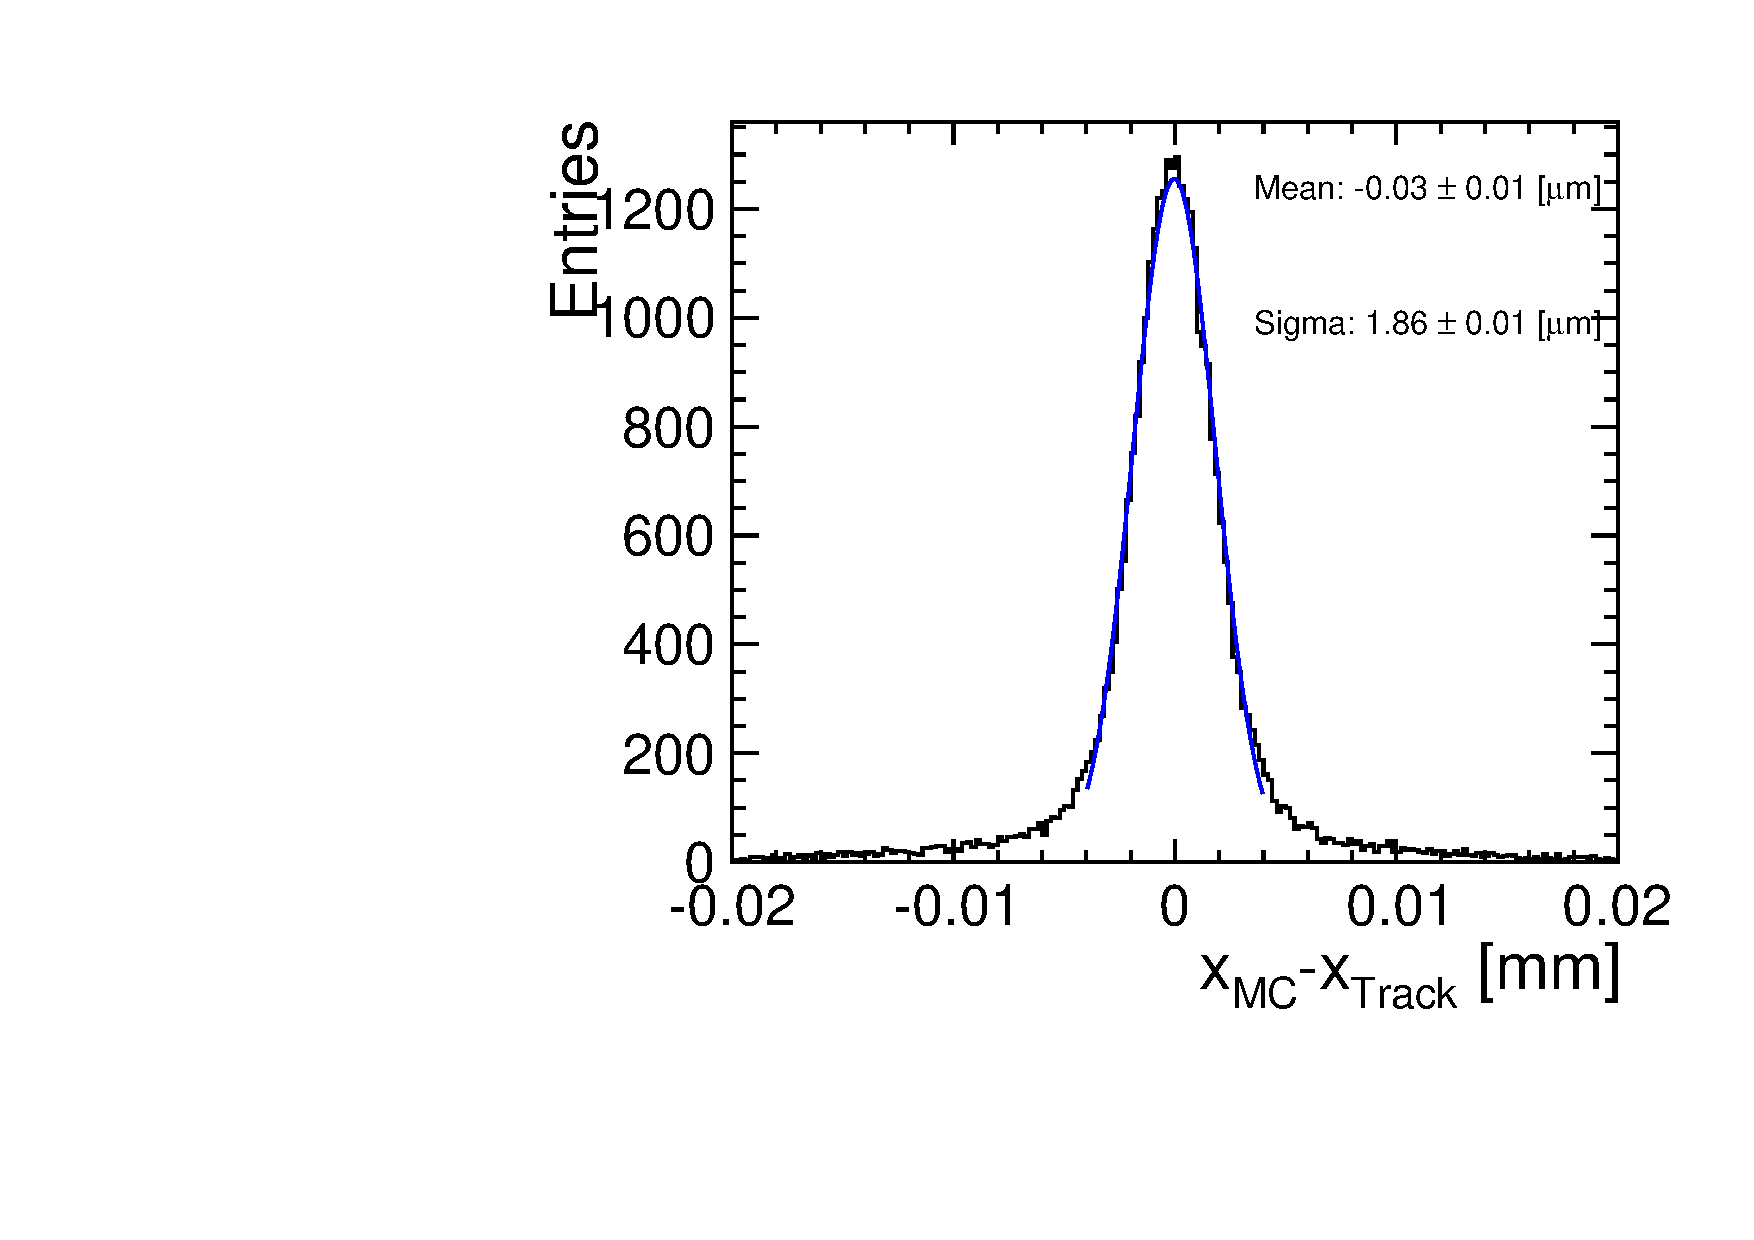
\includegraphics[width=\textwidth]{figures/Telescope/Unbiased_trackRes_DUT_x.pdf}
    \caption{}
  \end{subfigure}\hfill
  \begin{subfigure}[b]{0.45\textwidth}
    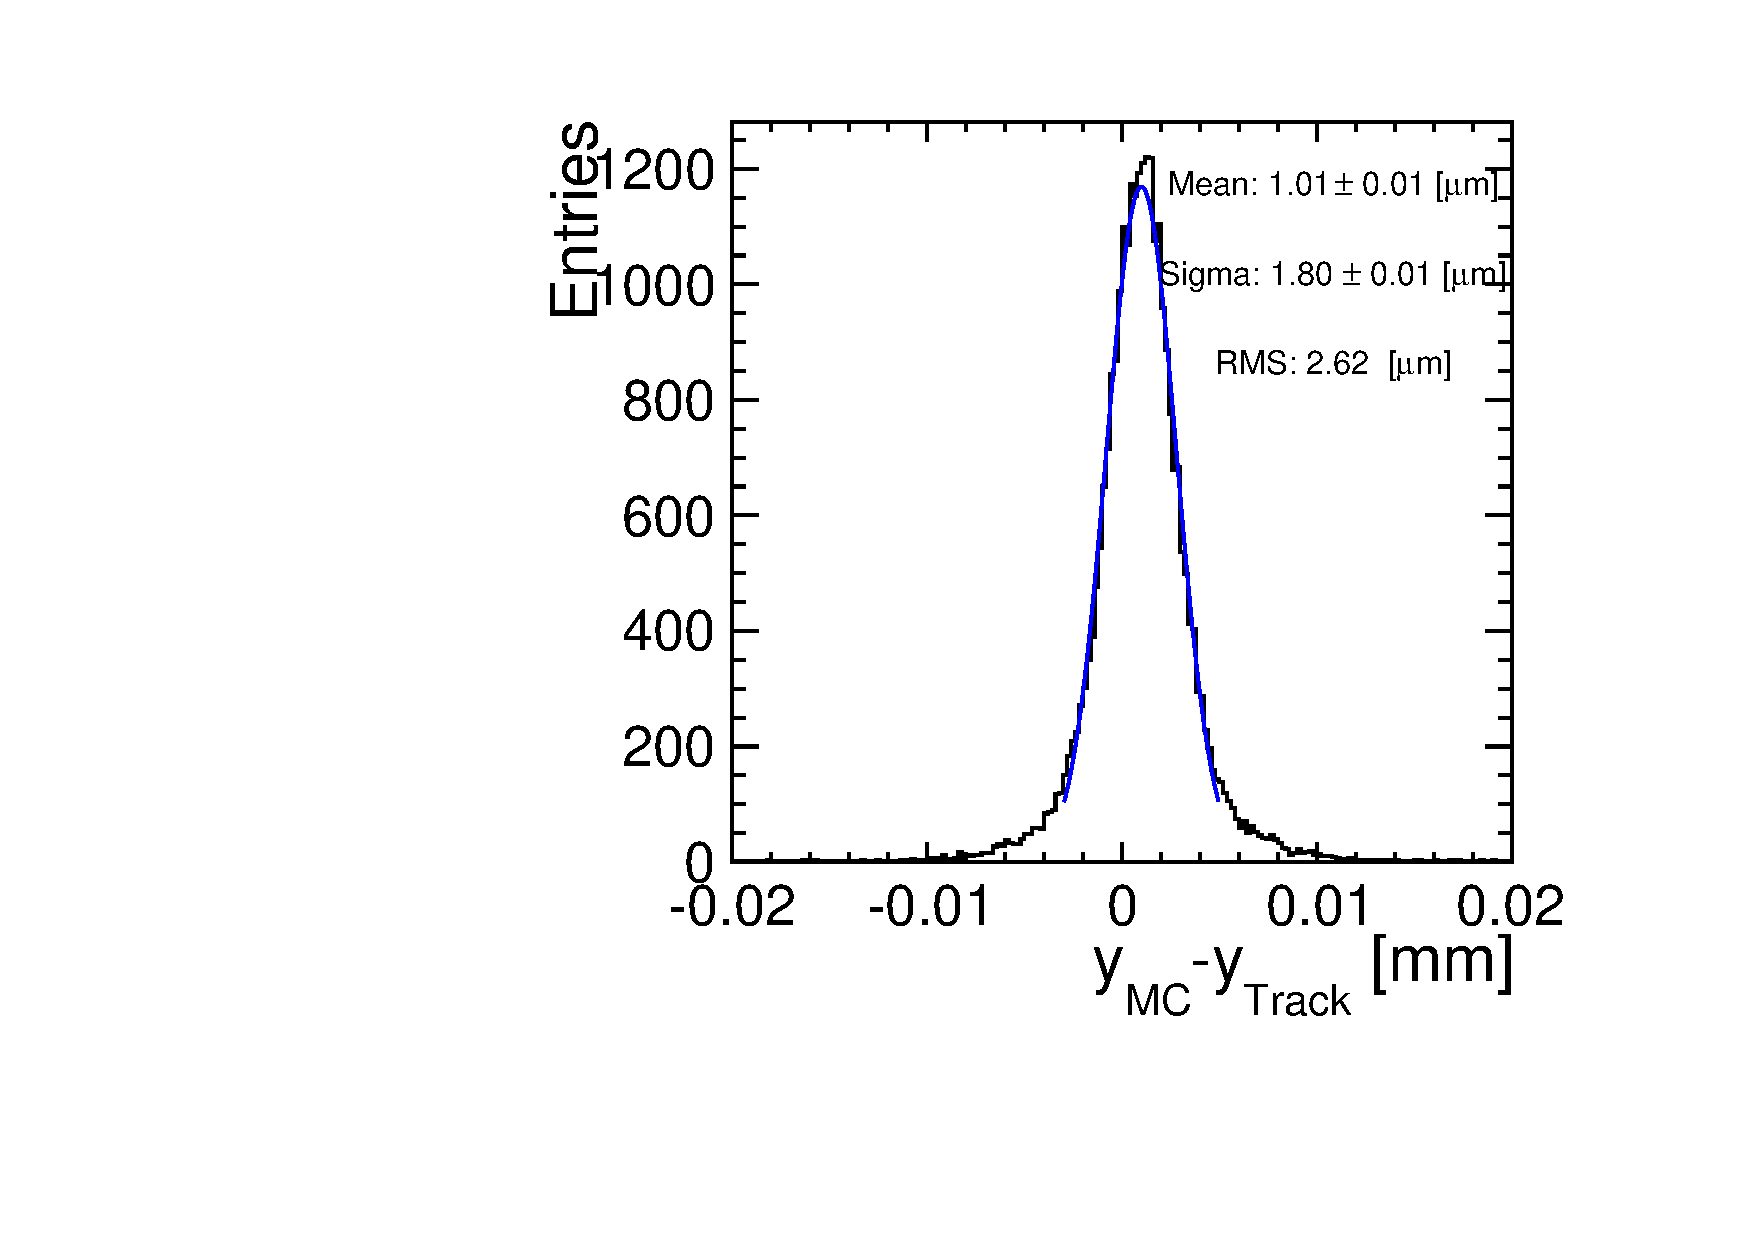
\includegraphics[width=\textwidth]{figures/Telescope/Unbiased_trackRes_DUT_y.pdf}
    \caption{}
  \end{subfigure}
  \caption{The track residuals on the DUT comparing the reconstructed
    track position to the true position of the particles obtained from
    \textsc{Geant4} in AllPix simulations in (a) x and (b) y
    directions.}
  \label{fig:DUT_MC_track}
\end{figure}


The standard deviation of the distributions is less than $2\,\micron$
when fitted by a Gaussian on the central $95.5\%$ of the residual
distribution. The RMS of the residuals is slightly higher than
$2\,\micron$ due to the tails of the distribution. A more strict cut
on the $\chi^2$/NDF discards tracks in the tails and reduces the RMS
of the distribution but also causes loss of statistics.

%% In the y-direction, the residuals show a shift of
%% $\sim1\,\micron$. This can be explained to the fact that in the
%% y-direction, the three planes before the DUT are rotated in an
%% asymmetric way compared to the three other planes after the DUT in the
%% Timepix3 telescope. Due to the rotation of the planes, the
%% reconstructed hit is biased towards higher y values for the planes
%% before and after the DUT. Therefore, the reconstructed track is also
%% biased towards higher y values. In the x-direction, the telescope
%% planes are rotated in a symmetric way. For the planes before the DUT,
%% the reconstructed hits are biased towards higher x values whereas for
%% the telescope planes after the DUT, the reconstructed hits are biased
%% towards lower x values. At the DUT position, the shift in the track
%% position is annihilated and no disalignement is observed at the
%% position of the DUT in the x direction. The shift in y-direction can
%% be corrected while aligning the DUT.


The tracking resolution on the DUT as a function of the
x\textsubscript{MC} and y\textsubscript{MC} positions is shown in
\cref{fig:DUT_MC_track_2D}. The resolution on the DUT does not depend
on the position of the track. This confirms the coherence between the
geometry description in the AllPix simulations and the EUTelescope
reconstruction. The shape of these distributions is due to the beam
profile which is more focused in the middle of the sensors.

\begin{figure}[htbp] \centering
  \begin{subfigure}[b]{0.45\textwidth}
    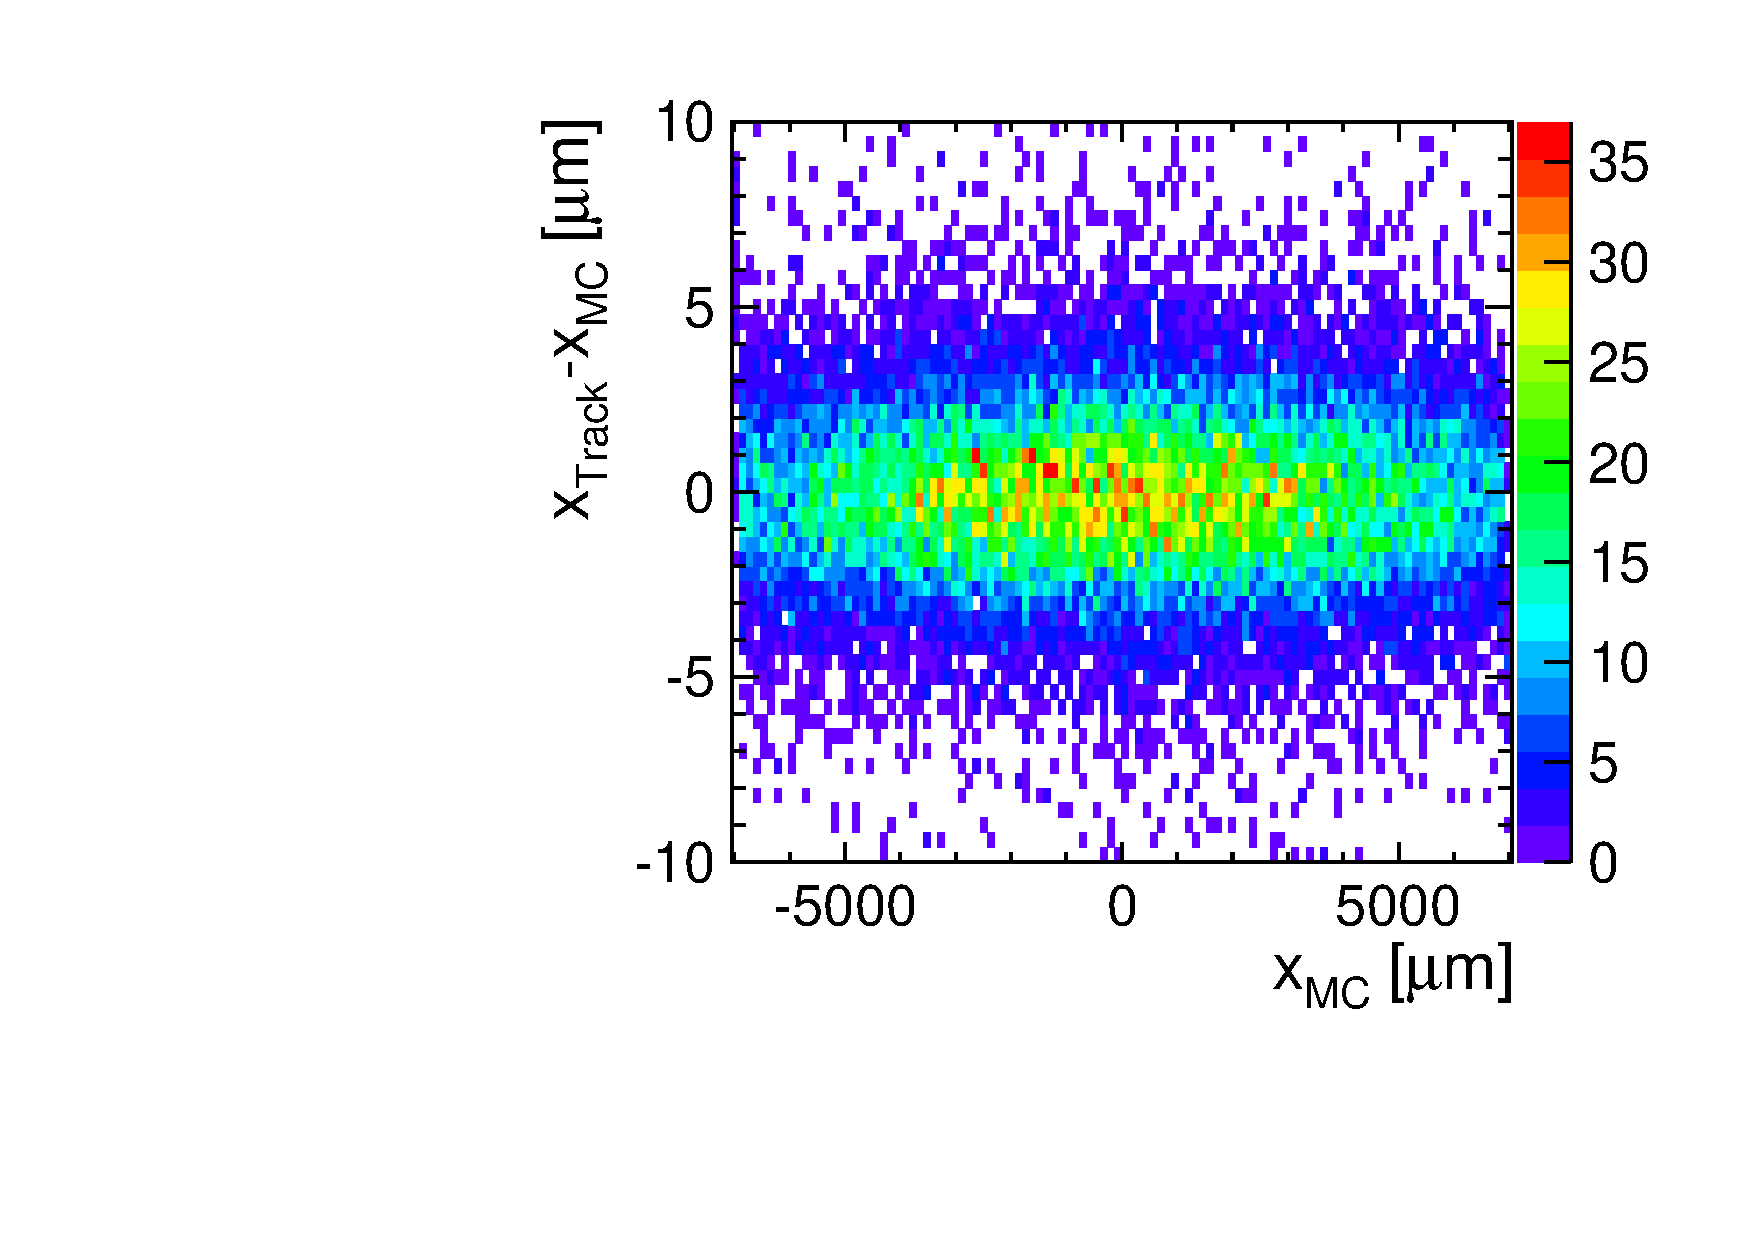
\includegraphics[width=\textwidth]{figures/Telescope/Unbiased_trackRes_DUT_x_2D.pdf}
    \caption{}
  \end{subfigure}\hfill
  \begin{subfigure}[b]{0.45\textwidth}
    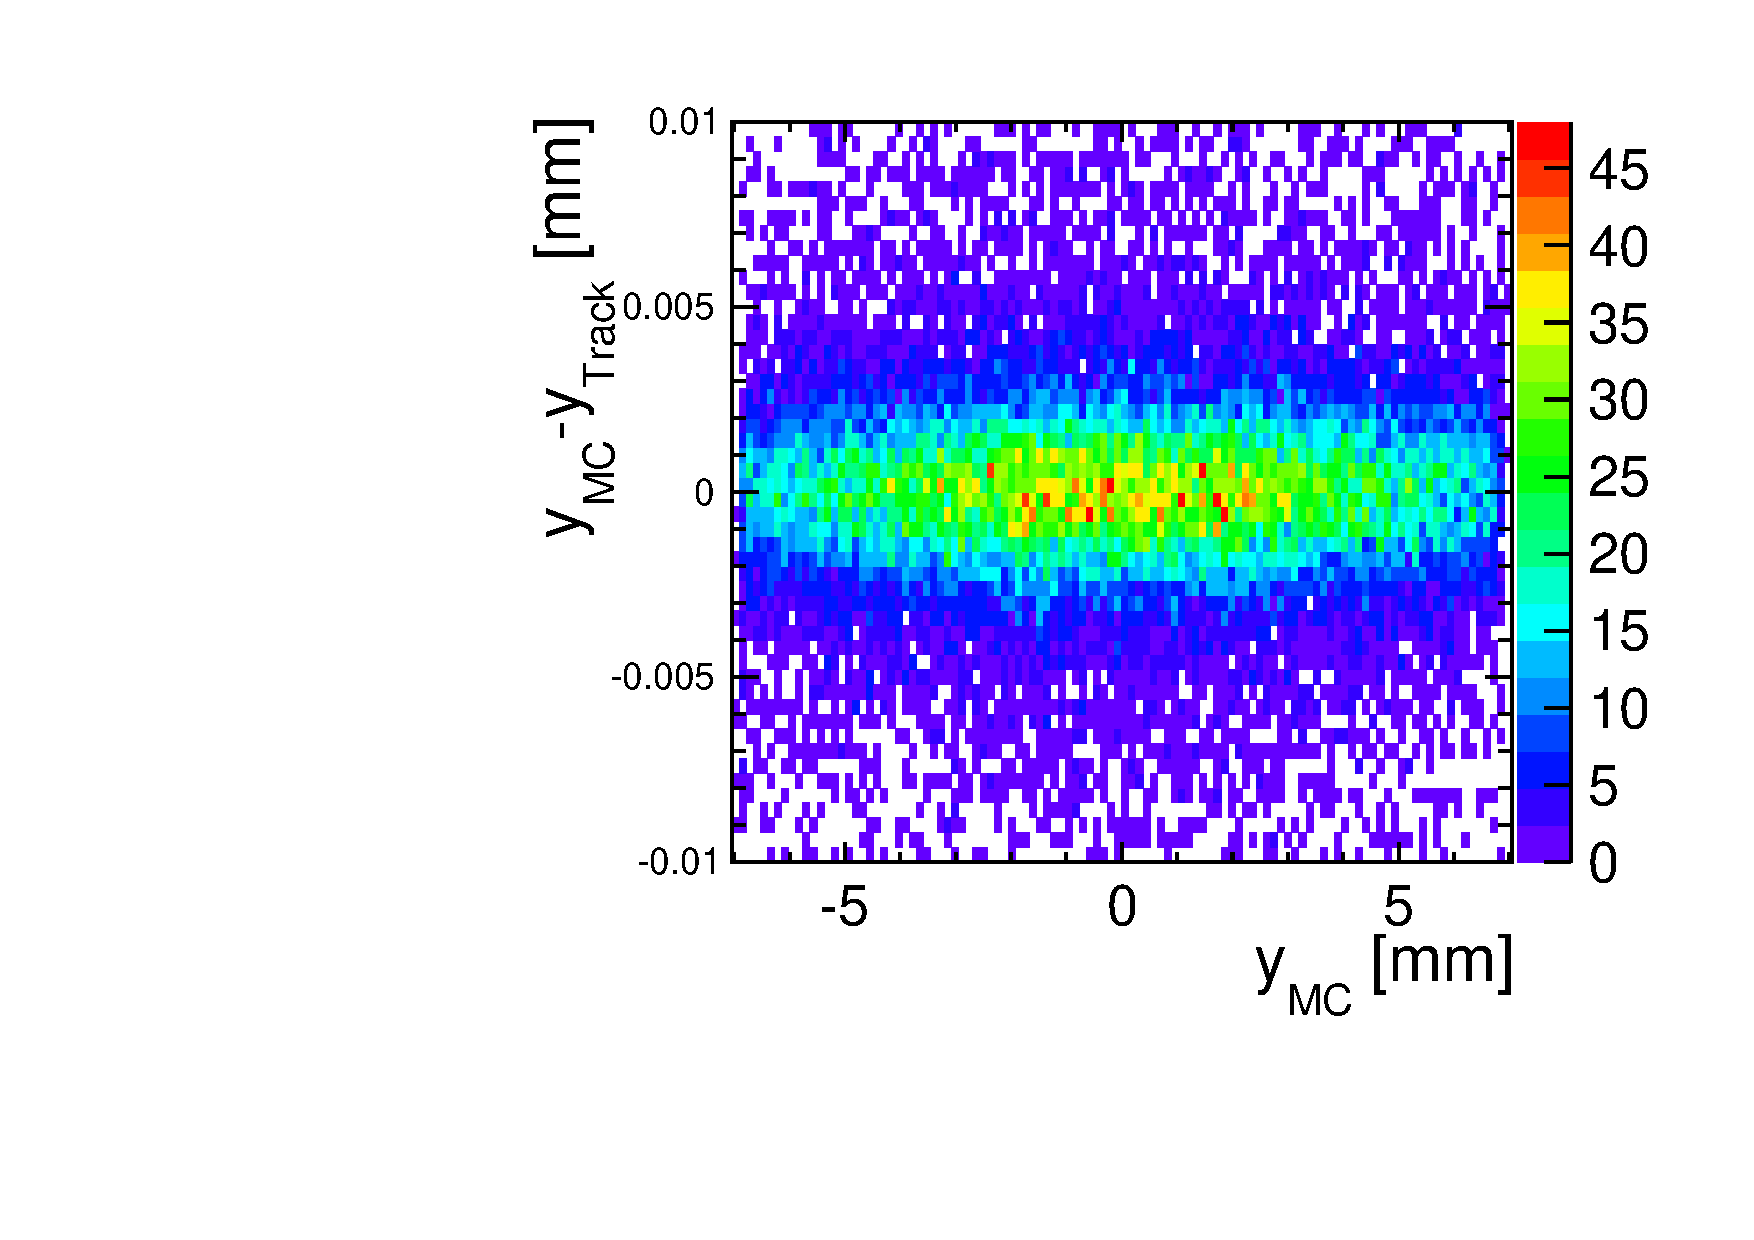
\includegraphics[width=\textwidth]{figures/Telescope/Unbiased_trackRes_DUT_y_2D.pdf}
    \caption{}
  \end{subfigure}
  \caption{The tracking resolution on the DUT in (a) x and (b) y
    directions as a function of the MC position.}
  \label{fig:DUT_MC_track_2D}
\end{figure}




%% --------------------------------------------- %%
\section{Summary}
\label{sec:Summary_Telescope}

The simulations confirm that the Timepix3 telescope allows for a
high-resolution track reconstruction on the DUT
($\sim2\,\micron$). This telescope is therefore suited for in-pixel
studies and testing of DUTs with high resolution constraints as
required for the CLIC vertex detector. In the following, the Timepix3
telescope is used to precisely characterise the performance of thin
sensors.

%% \begin{table}[htbp]
%%   \centering
%%   \caption{A summary of the measured telescope performance.}
%%   \label{tab:SummaryOfResolutions}
%%   \begin{tabular}{ccc}
%%     \toprule
%%     $\sigma$\textsubscript{int} [$\micron$] & $\sigma$\textsubscript{x,DUT} [$\micron$] & $\sigma$\textsubscript{y,DUT} [$\micron$]\\
%%     \midrule
%%     2.6 & 1.94 & 1.80 \\
%%     \bottomrule
%%   \end{tabular}
%% \end{table}


%% --------------------------------------------- %%

